\section{Results}
\label{sec:results}

\subsection{Parameter settings}

In all of the following results, we use a suite size of 1200 (that is, 1200
independent simulations with different random number seeds for \textit{each}
combination of distinct independent variable values) and run each simulation
for 400 iterations. We set $V_N=20$ voters, $C_N=3$ candidates, $I_N=3$ issues,
$p_e=.2$ edge probability, and $E=50$ for eight consecutive elections in the
400 iteration time period.

\subsection{Multiple chasers impede one another}

Using the default voting algorithm distribution ($\frac{1}{3}$ rational,
$\frac{1}{3}$ party, $\frac{1}{6}$ F\&F1, $\frac{1}{6}$ F\&F2)
When only one of three candidates is chasing votes, it reaches its ``sweet
spot'' early on, and quickly encounters diminishing returns to further chasing.
When two candidates are chasing, they take longer to reach their equilibrium.
(See Figure~\ref{one_vs_two_chasers}.) We speculate that this is because the
chasers are interfering with one another as they court voters in opinion space,
dampening the gains of their rival by moving into regions that might have been
unspoken for.

\begin{figure}[ht]
\centering
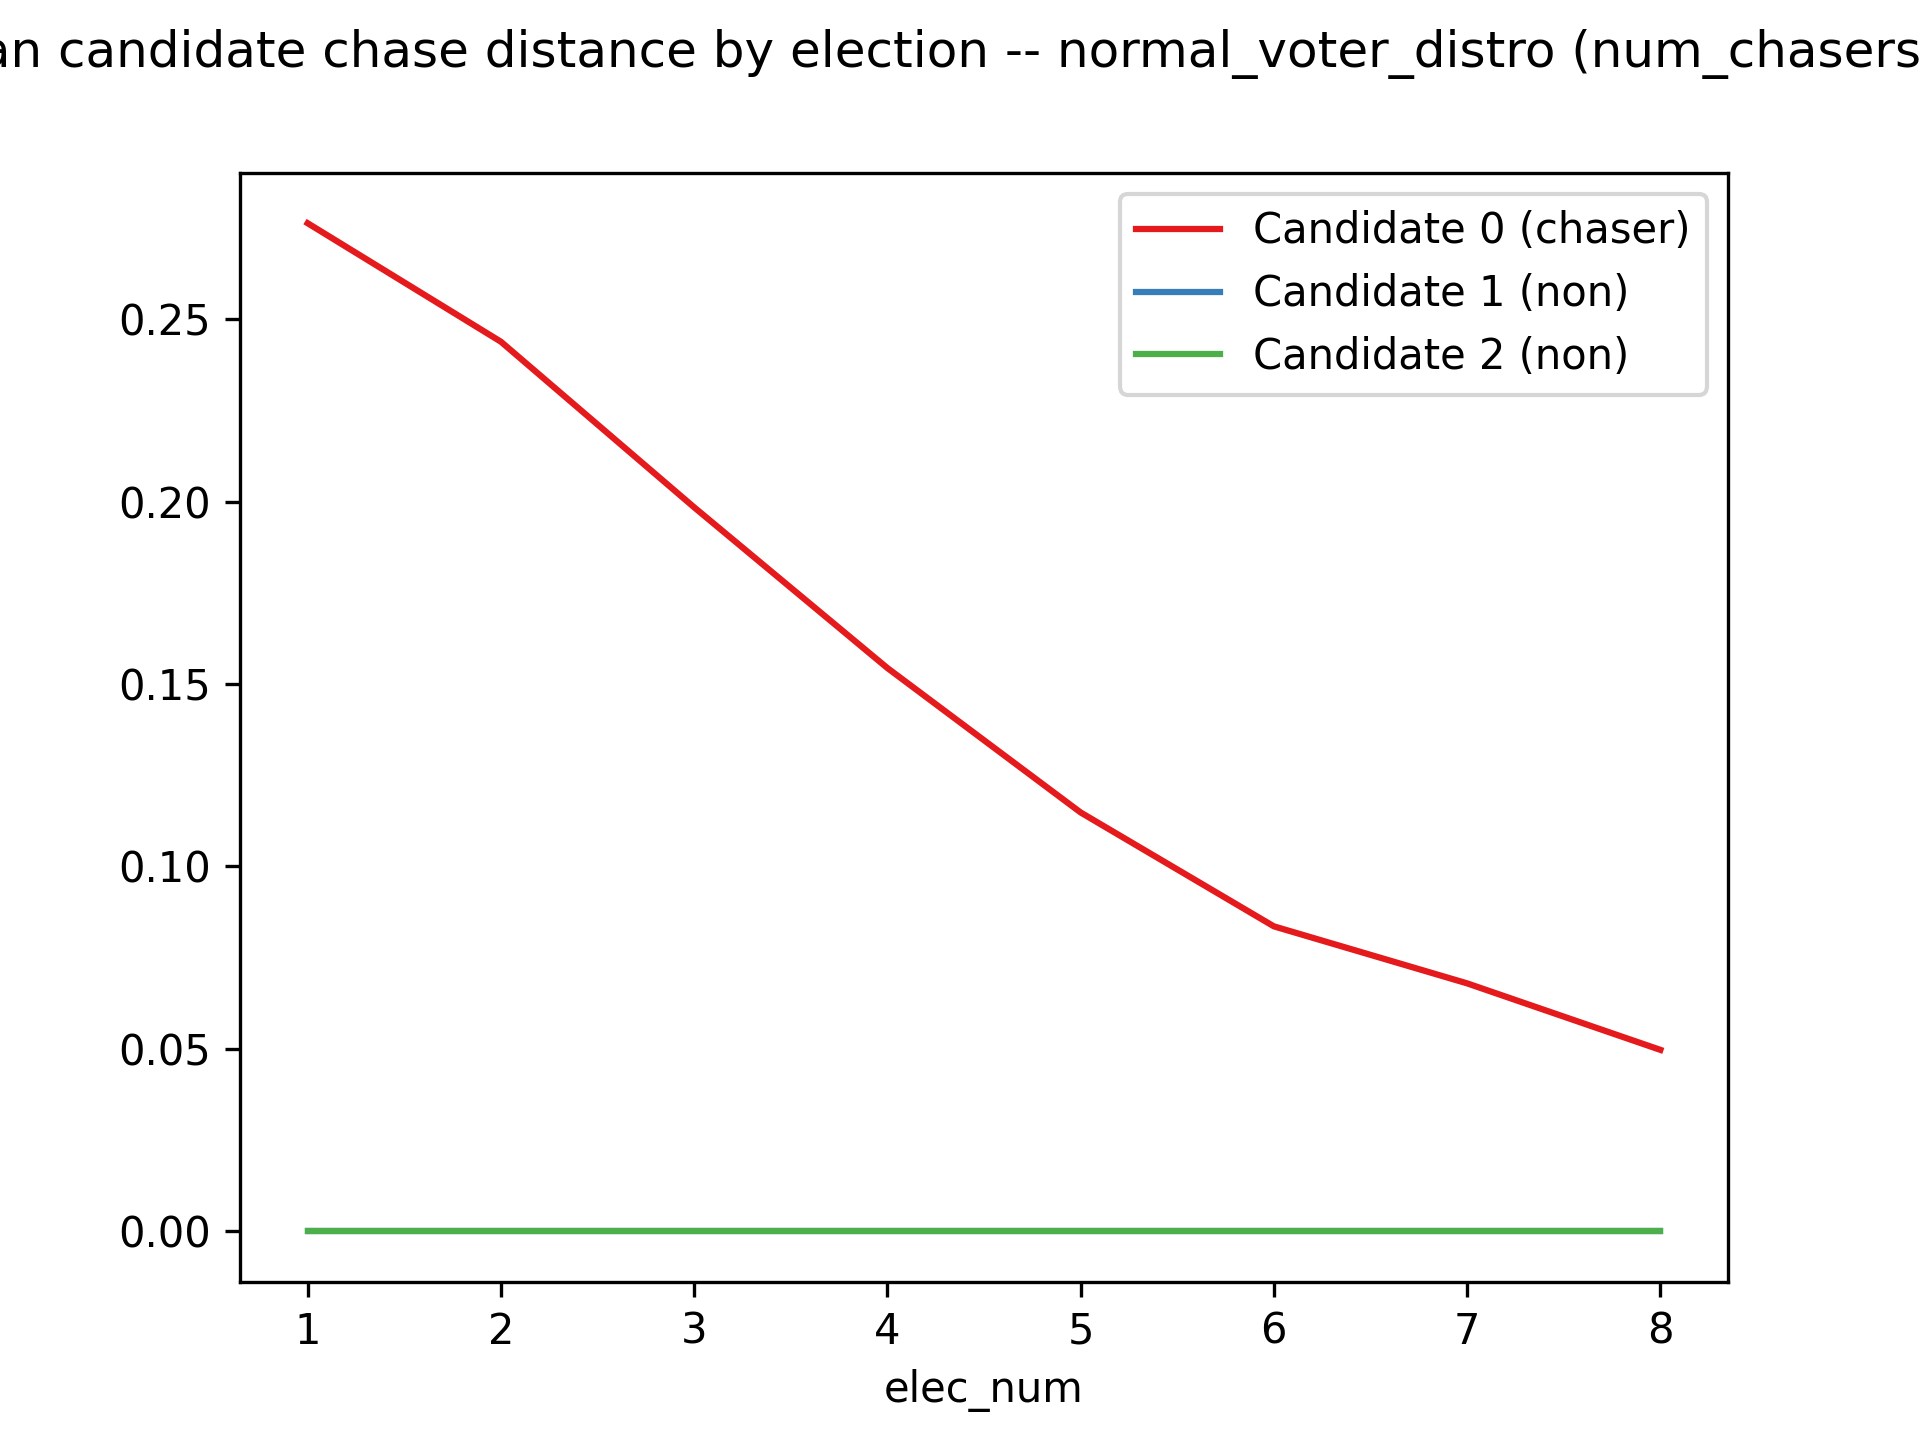
\includegraphics[width=0.45\textwidth]{assets/one_chaser_maxes_out_soon.png}
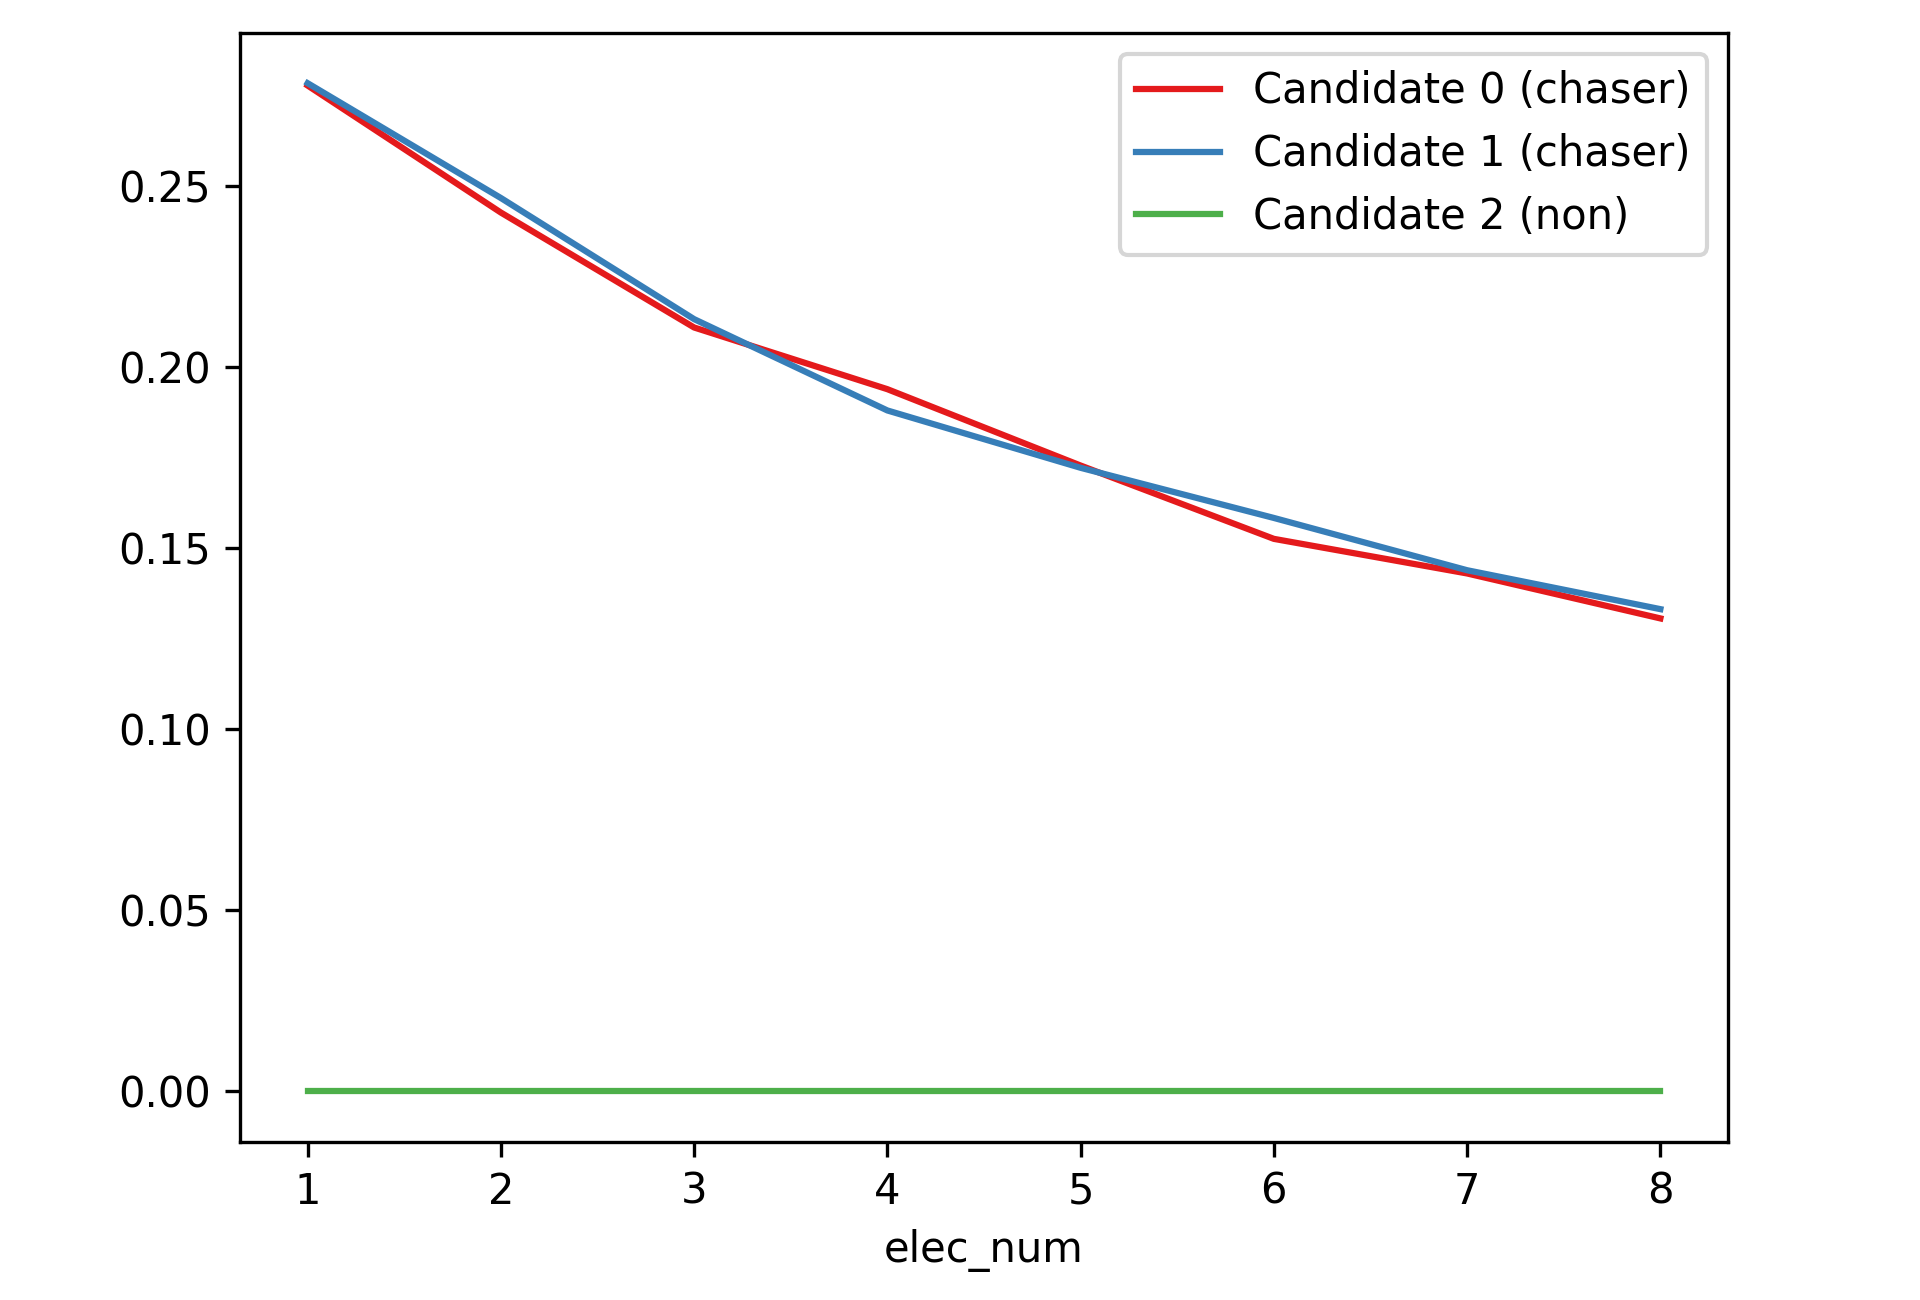
\includegraphics[width=0.45\textwidth]{assets/two_chasers_max_out_later.png}
\caption{A single chasing candidate maxes out its gains more quickly than two
competing chasers do.}
\label{one_vs_two_chasers}
\end{figure}

\subsection{Multiple chasers reduce one another's gains}

The above effect can be further illustrated by looking at how many elections
are actually won by chasing vs. non-chasing candidates.
Figure~\ref{chasing_winners} shows the proportion of elections won by each
candidate in a three-candidate race with one chaser (left side) and with two
(right side). (Error bars are 95\% confidence intervals for a proportion,
assuming normality.) As you can see, when only one candidate chases voters, it
has a tremendous advantage over the other candidates, and this advantage
increases the longer that the drifting/chasing mechanism continues. Two
chasers, however, interfere with one another such that each gets only a modest
benefit.

\begin{figure}[ht]
\centering
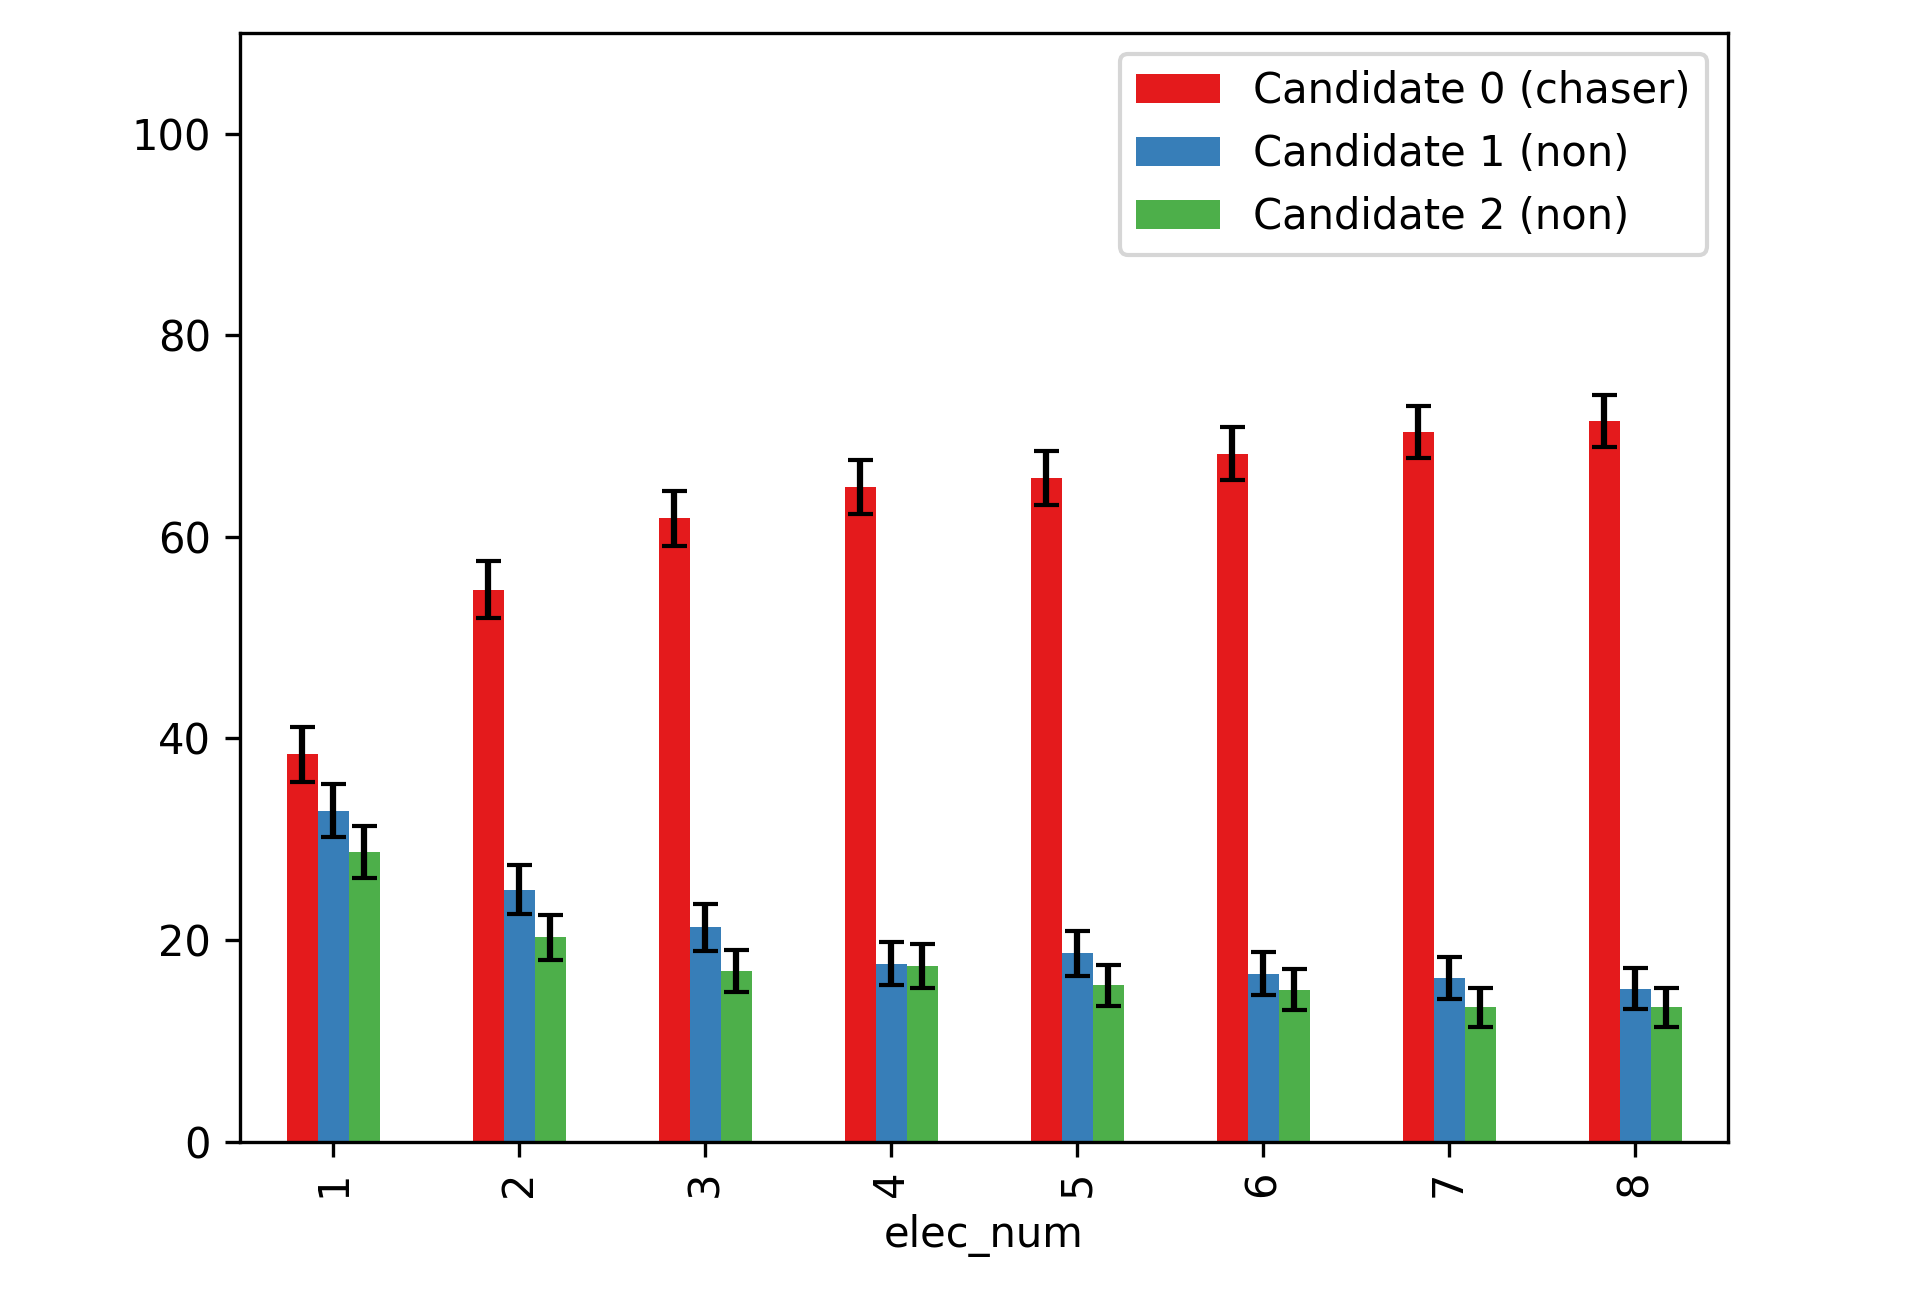
\includegraphics[width=0.45\textwidth]{assets/one_chaser_big_benefit.png}
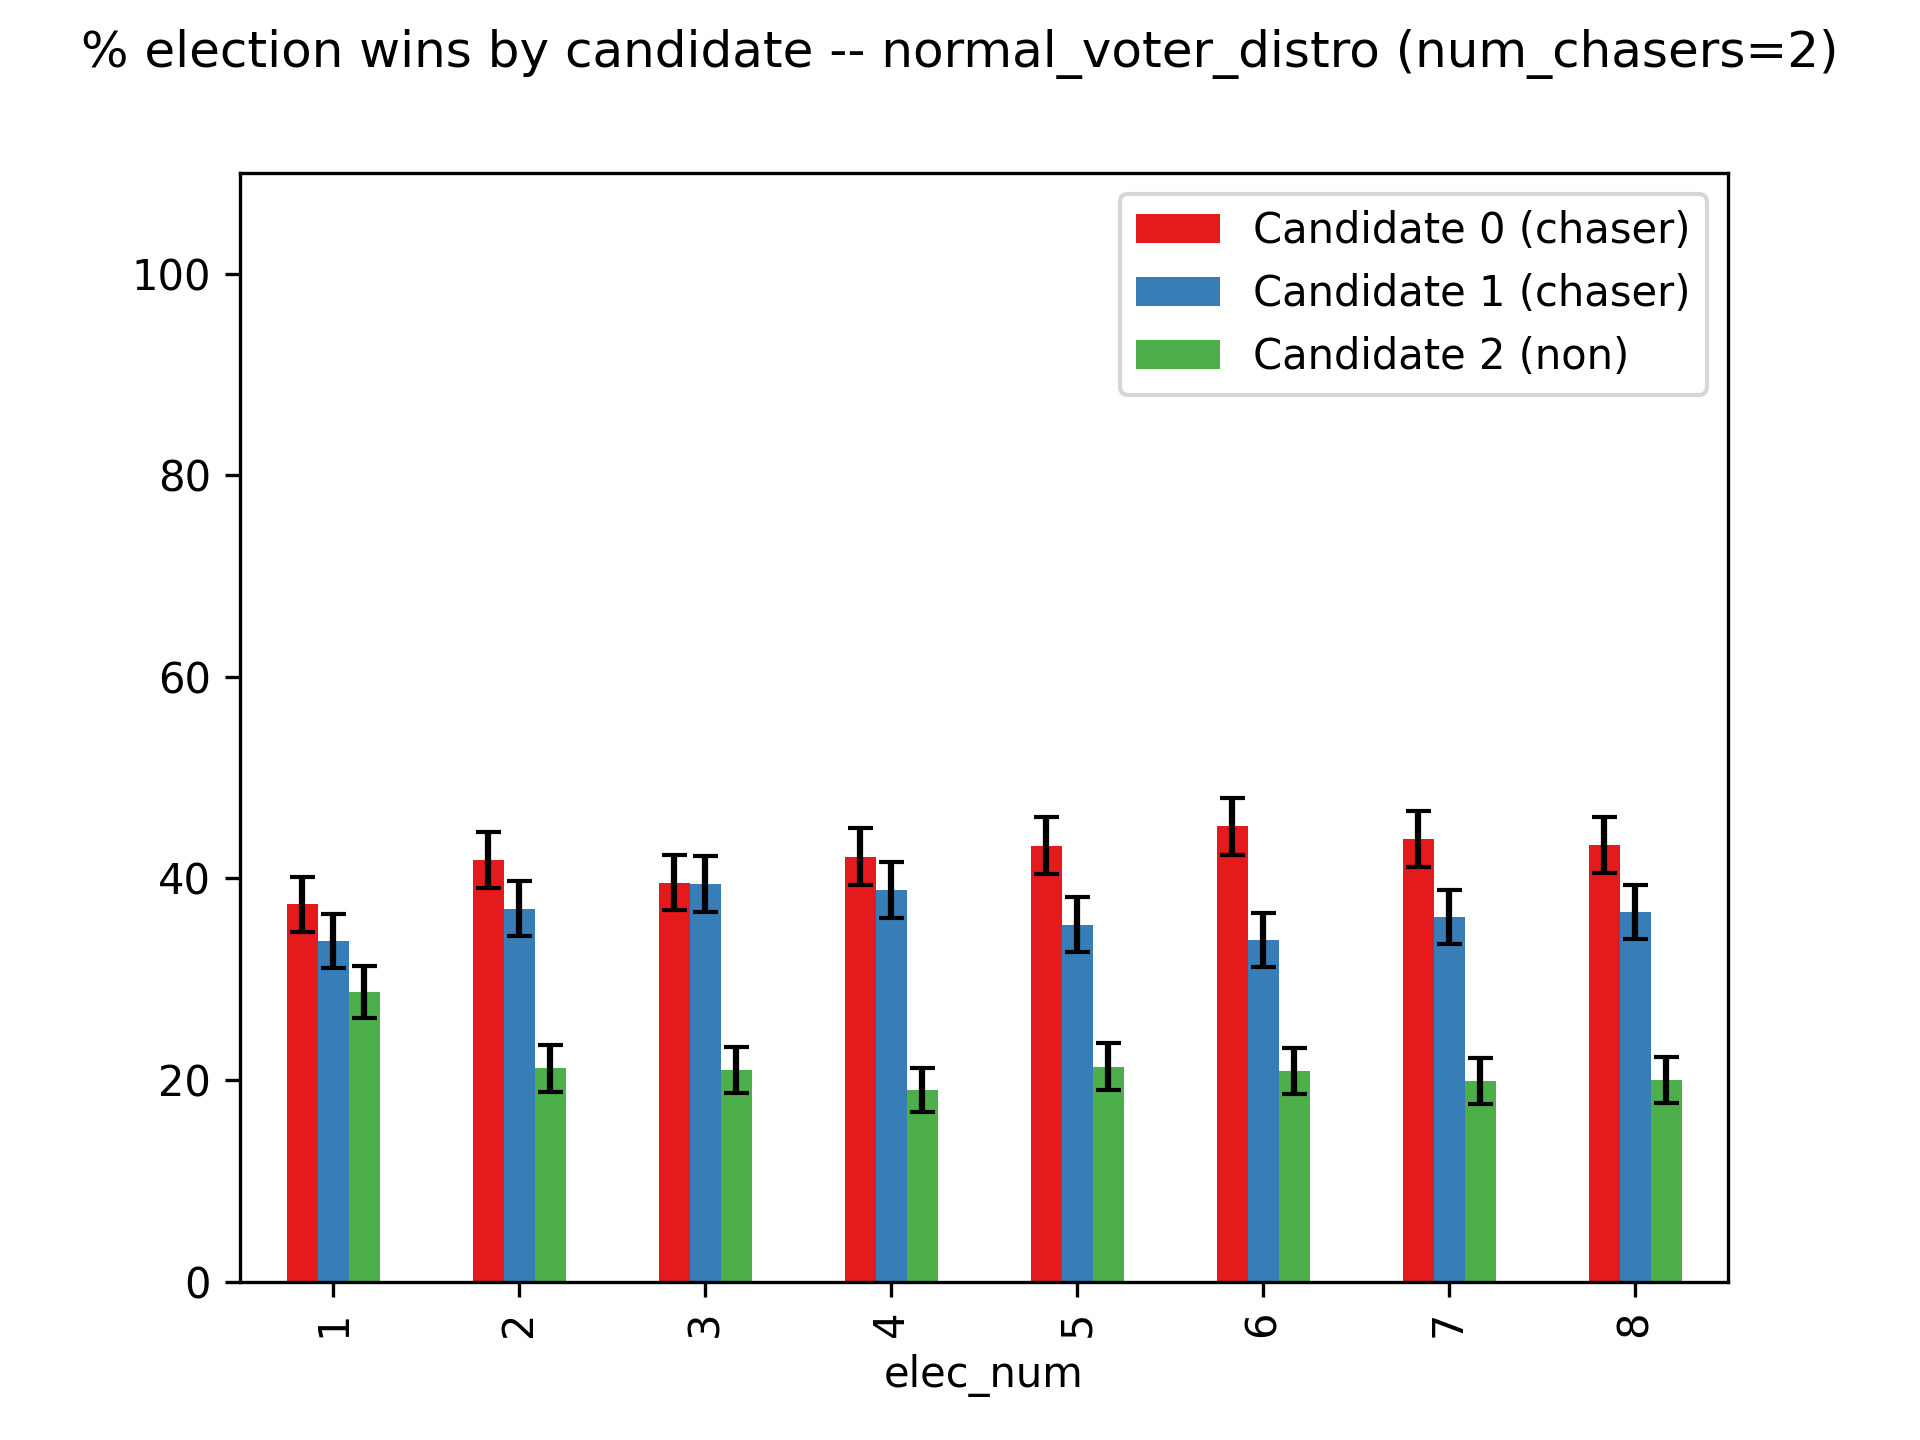
\includegraphics[width=0.45\textwidth]{assets/two_chasers_small_benefit.png}
\caption{Using the default voting algorithm distribution, a single chasing
candidate (red) has an enormous advantage over its competitors. If two
candidates (both red and blue) are chasing voters, however, neither gains
nearly as much benefit. (Note: the small advantages that red consistently has
over blue are an artifact of how the simulation handles ties -- it awards
victory to the lowest-numbered tied candidate. This is miniscule in comparison
with the main effect illustrated here, however.)}
\label{chasing_winners}
\end{figure}

\subsection{The impact of voting algorithm distribution}

All of the above results were obtained with the default voting algorithm
distribution ($\frac{1}{3}$ rational, $\frac{1}{3}$ party, $\frac{1}{6}$ F\&F1,
$\frac{1}{6}$ F\&F2) and it turns out they are highly sensitive to it. In an
electorate with \textit{no} rational voters, by contrast, chasers get little to
no benefit. They are trying to appeal to the issue positions of voters who will
not in fact be voting based on those positions. Chasing candidates have no
advantage even if there are many, or even all, F\&F voters. This is somewhat
surprising since F\&F voters do ``noisily'' vote based on their issue positions
(they consider only one of them, instead of all three). Compare
Figure~\ref{chasing_vs_distro} (the left side has all party-line voters, the
right side has all F\&F voters) with the left side of
Figure~\ref{chasing_winners} (which has the default voting algorithm
distribution) to see the difference.

\begin{figure}[ht]
\centering
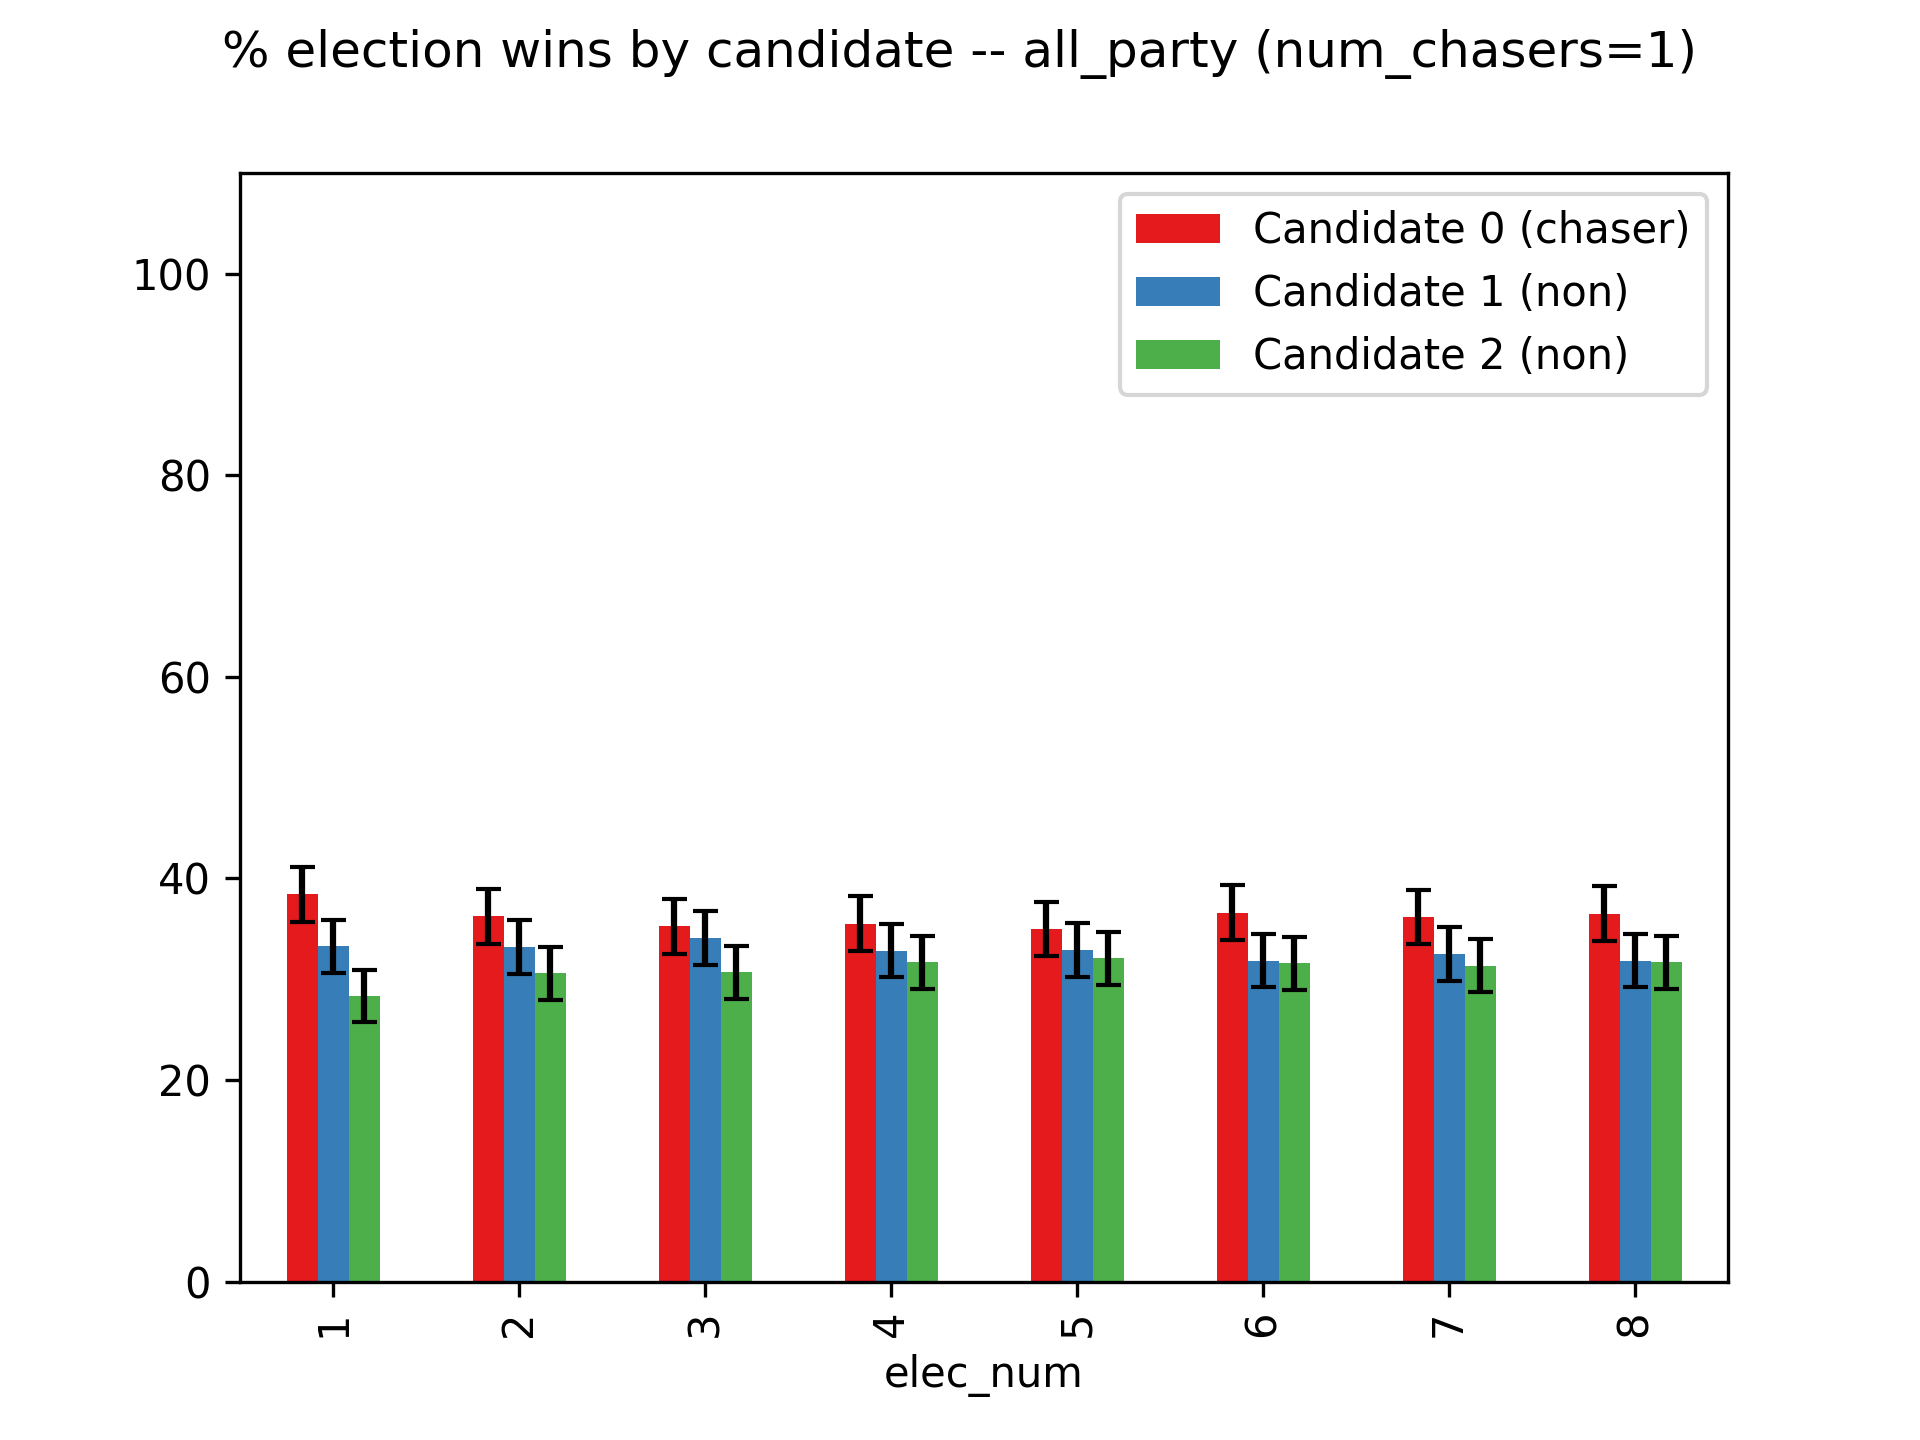
\includegraphics[width=0.45\textwidth]{assets/all_party_1_chaser_no_benefit.png}
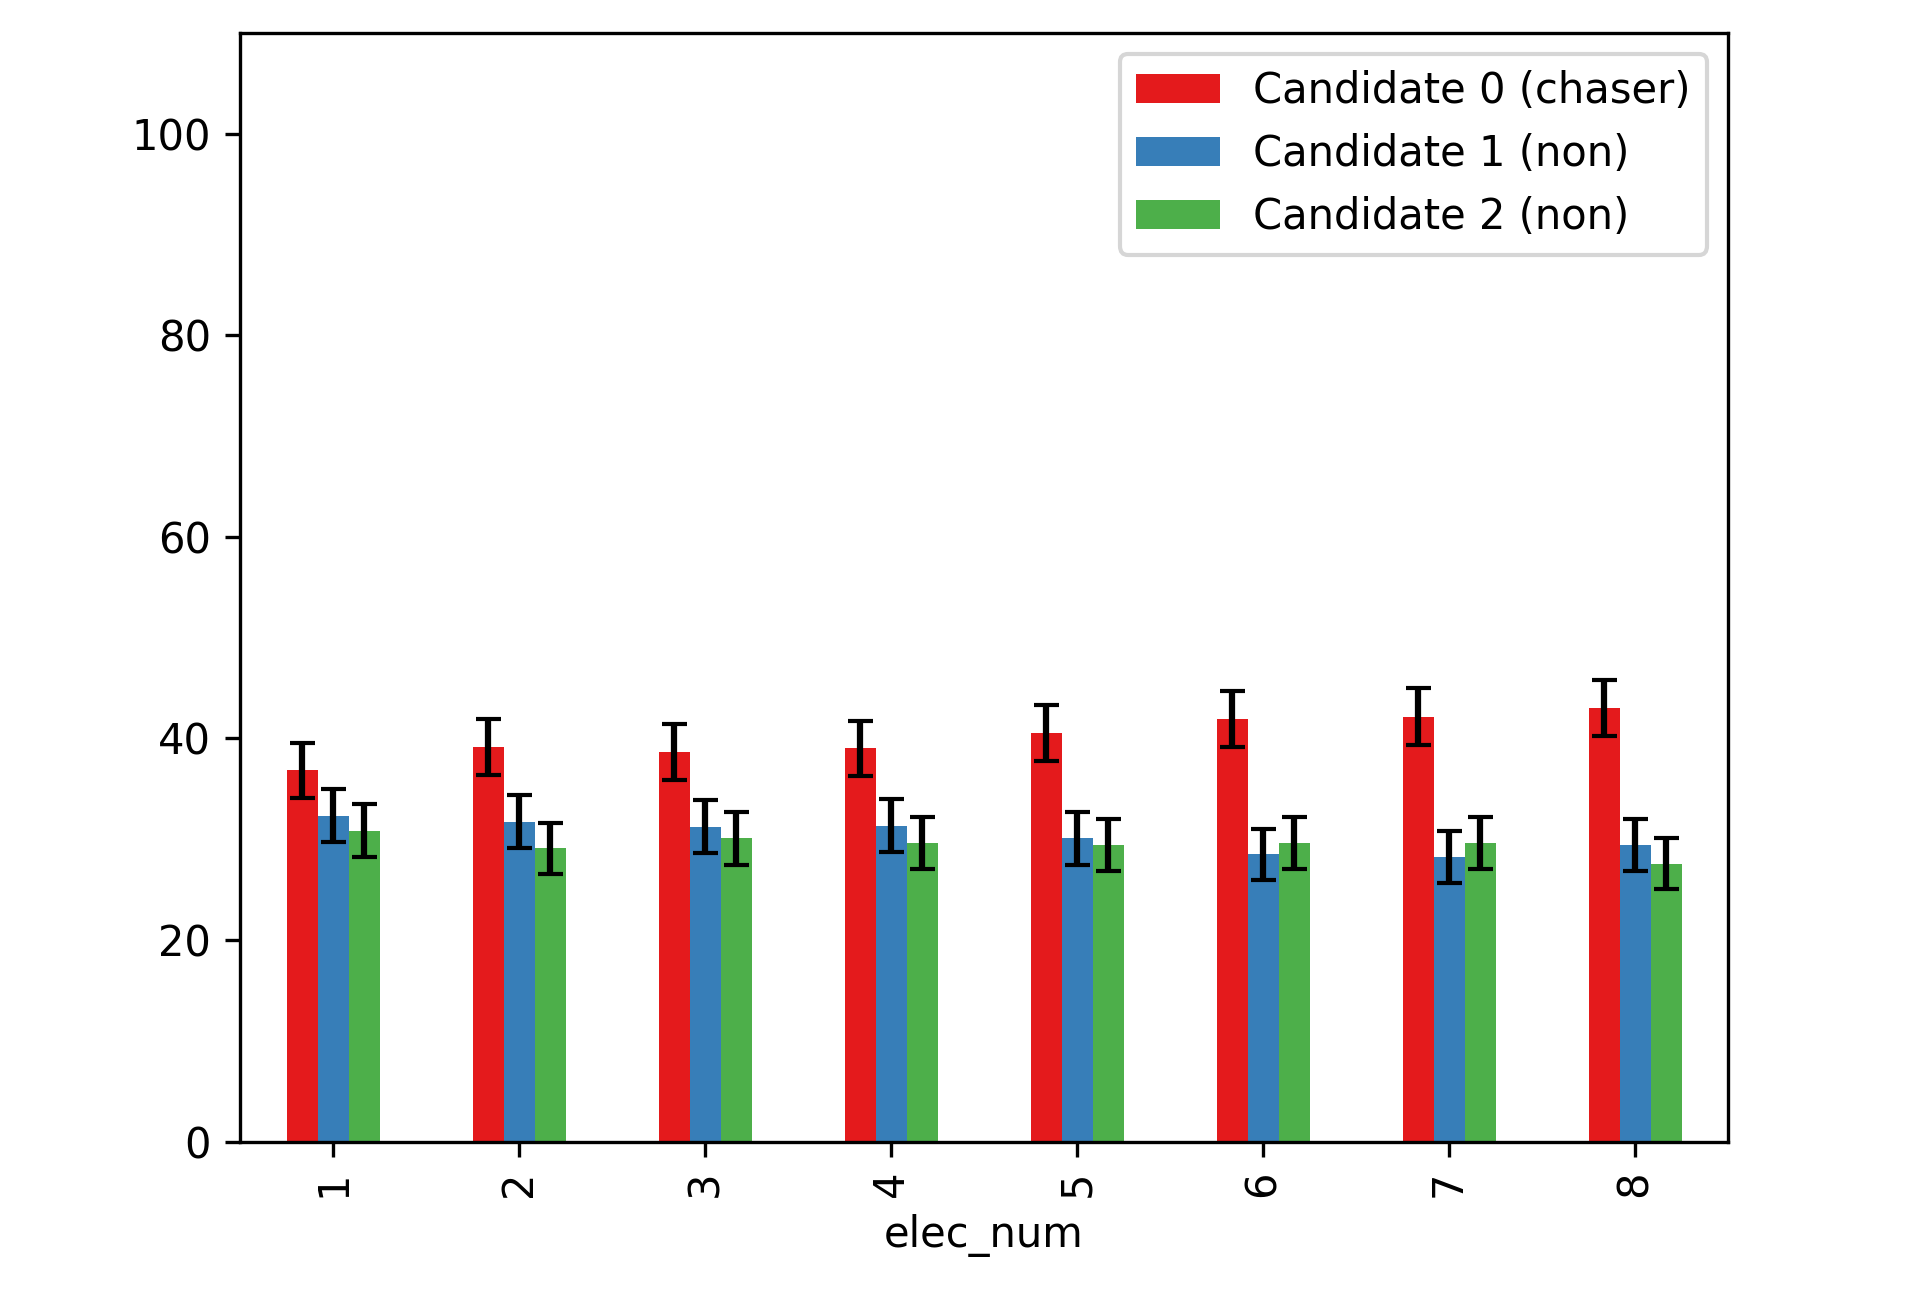
\includegraphics[width=0.45\textwidth]{assets/all_ff_chasers_no_benefit.png}
\caption{When the electorate is changed to have all party-line voters (left) or
all fast \& frugal voters (right), chasing candidates have little appreciable
advantage.}
\label{chasing_vs_distro}
\end{figure}

At the other extreme, an electorate of all rational voters gives the maximum
benefit to chasing candidates (see Figure~\ref{all_rat_chasers_benefit}). In
this scenario, even when two candidates are chasers, they do not interfere with
one another enough to nullify their effects -- both easily eclipse the single
non-chasing candidate (Figure~\ref{all_rat_chasers_benefit}, right side.)

\begin{figure}[ht]
\centering
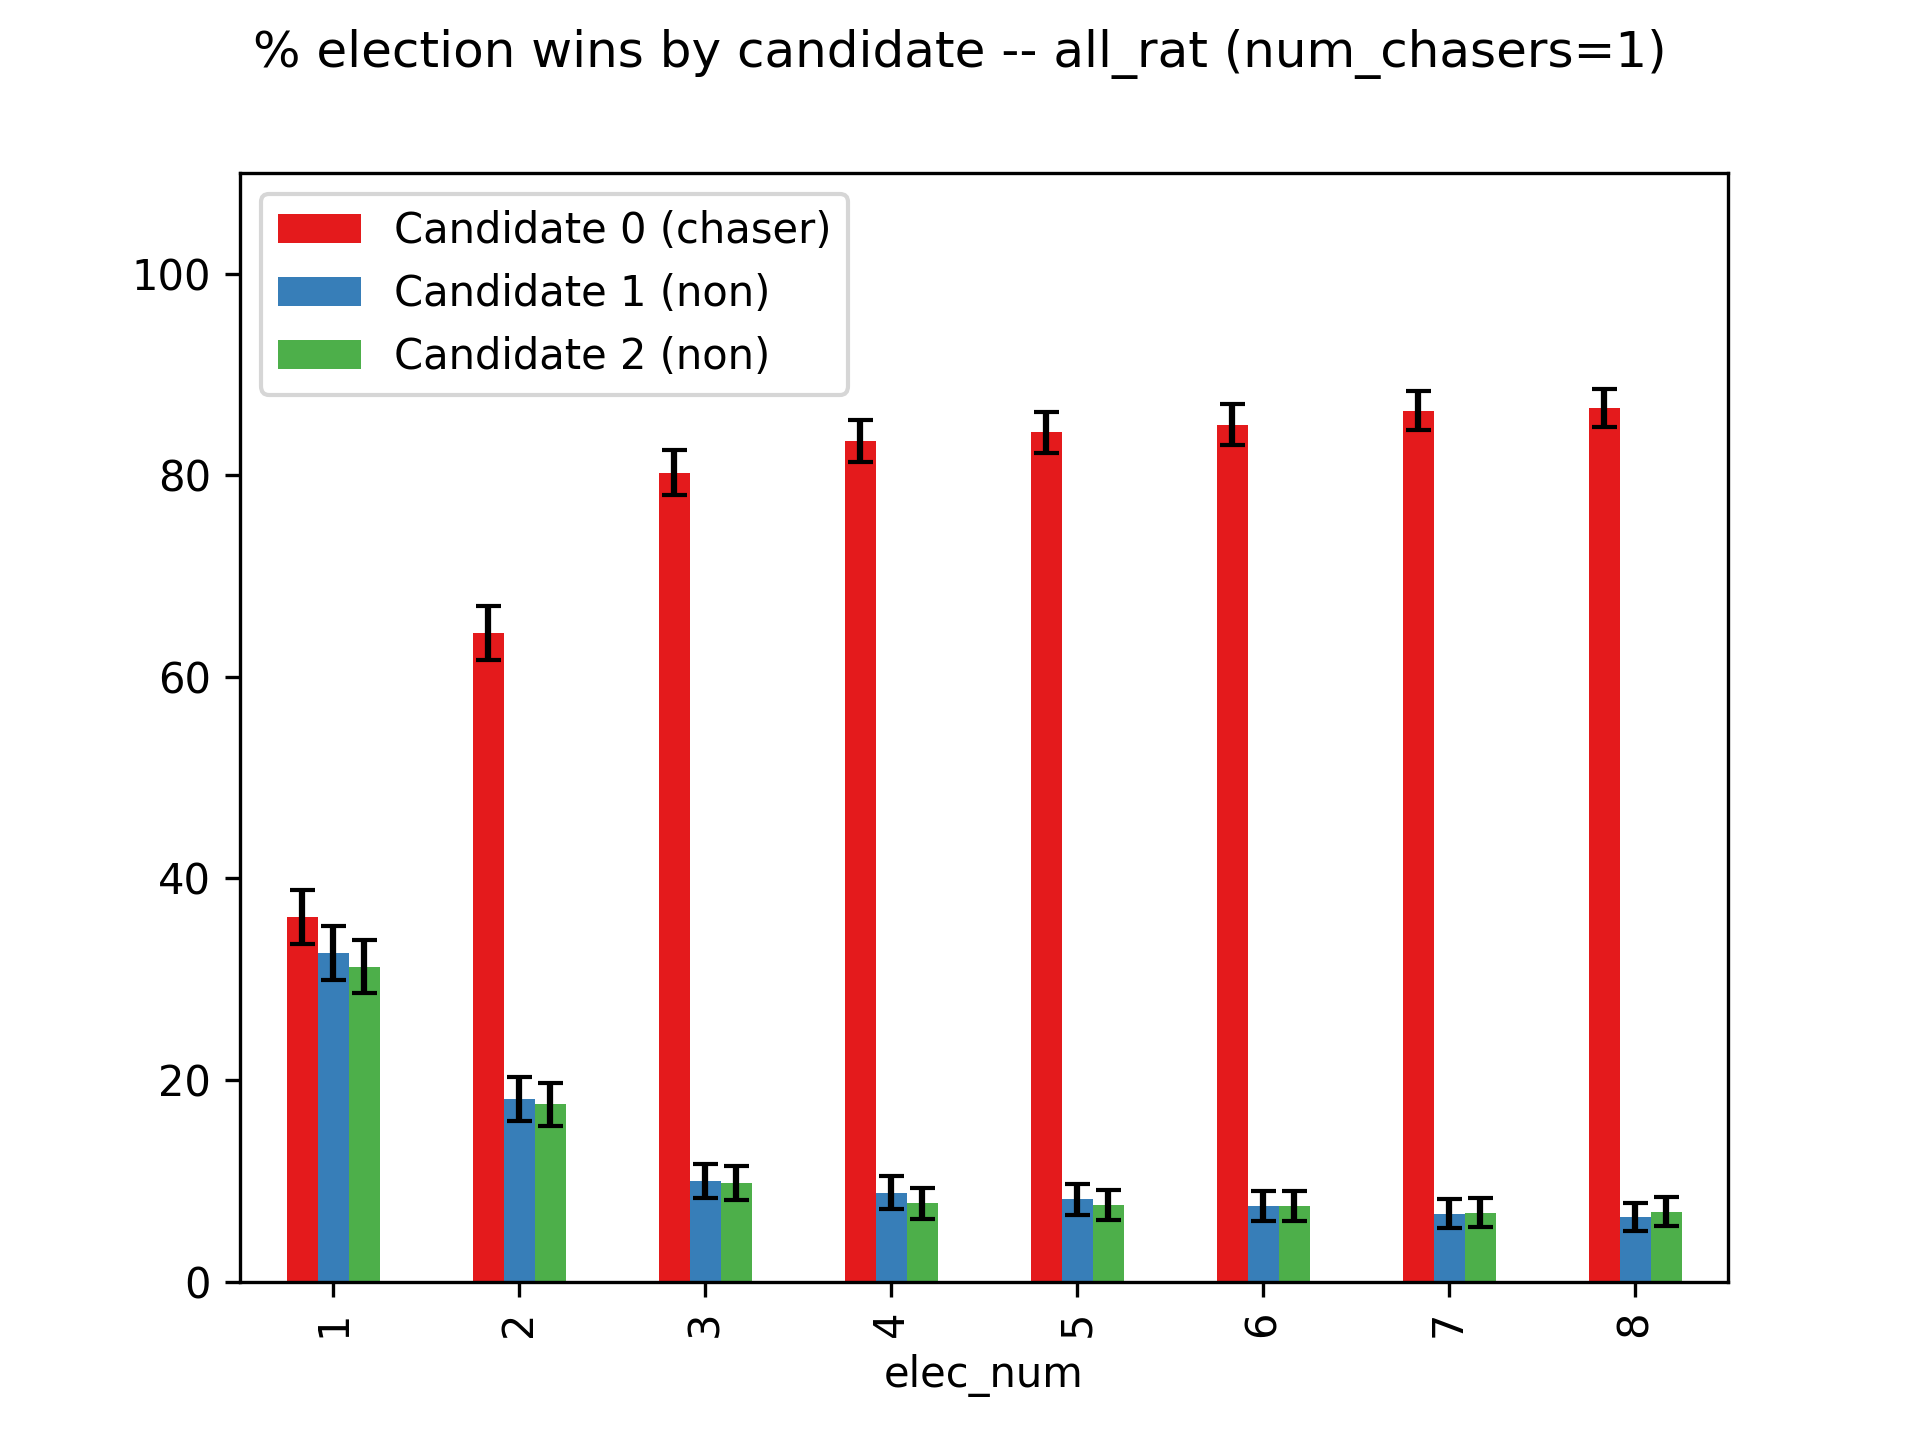
\includegraphics[width=0.45\textwidth]{assets/all_rat_one_chaser_even_bigger_benefit.png}
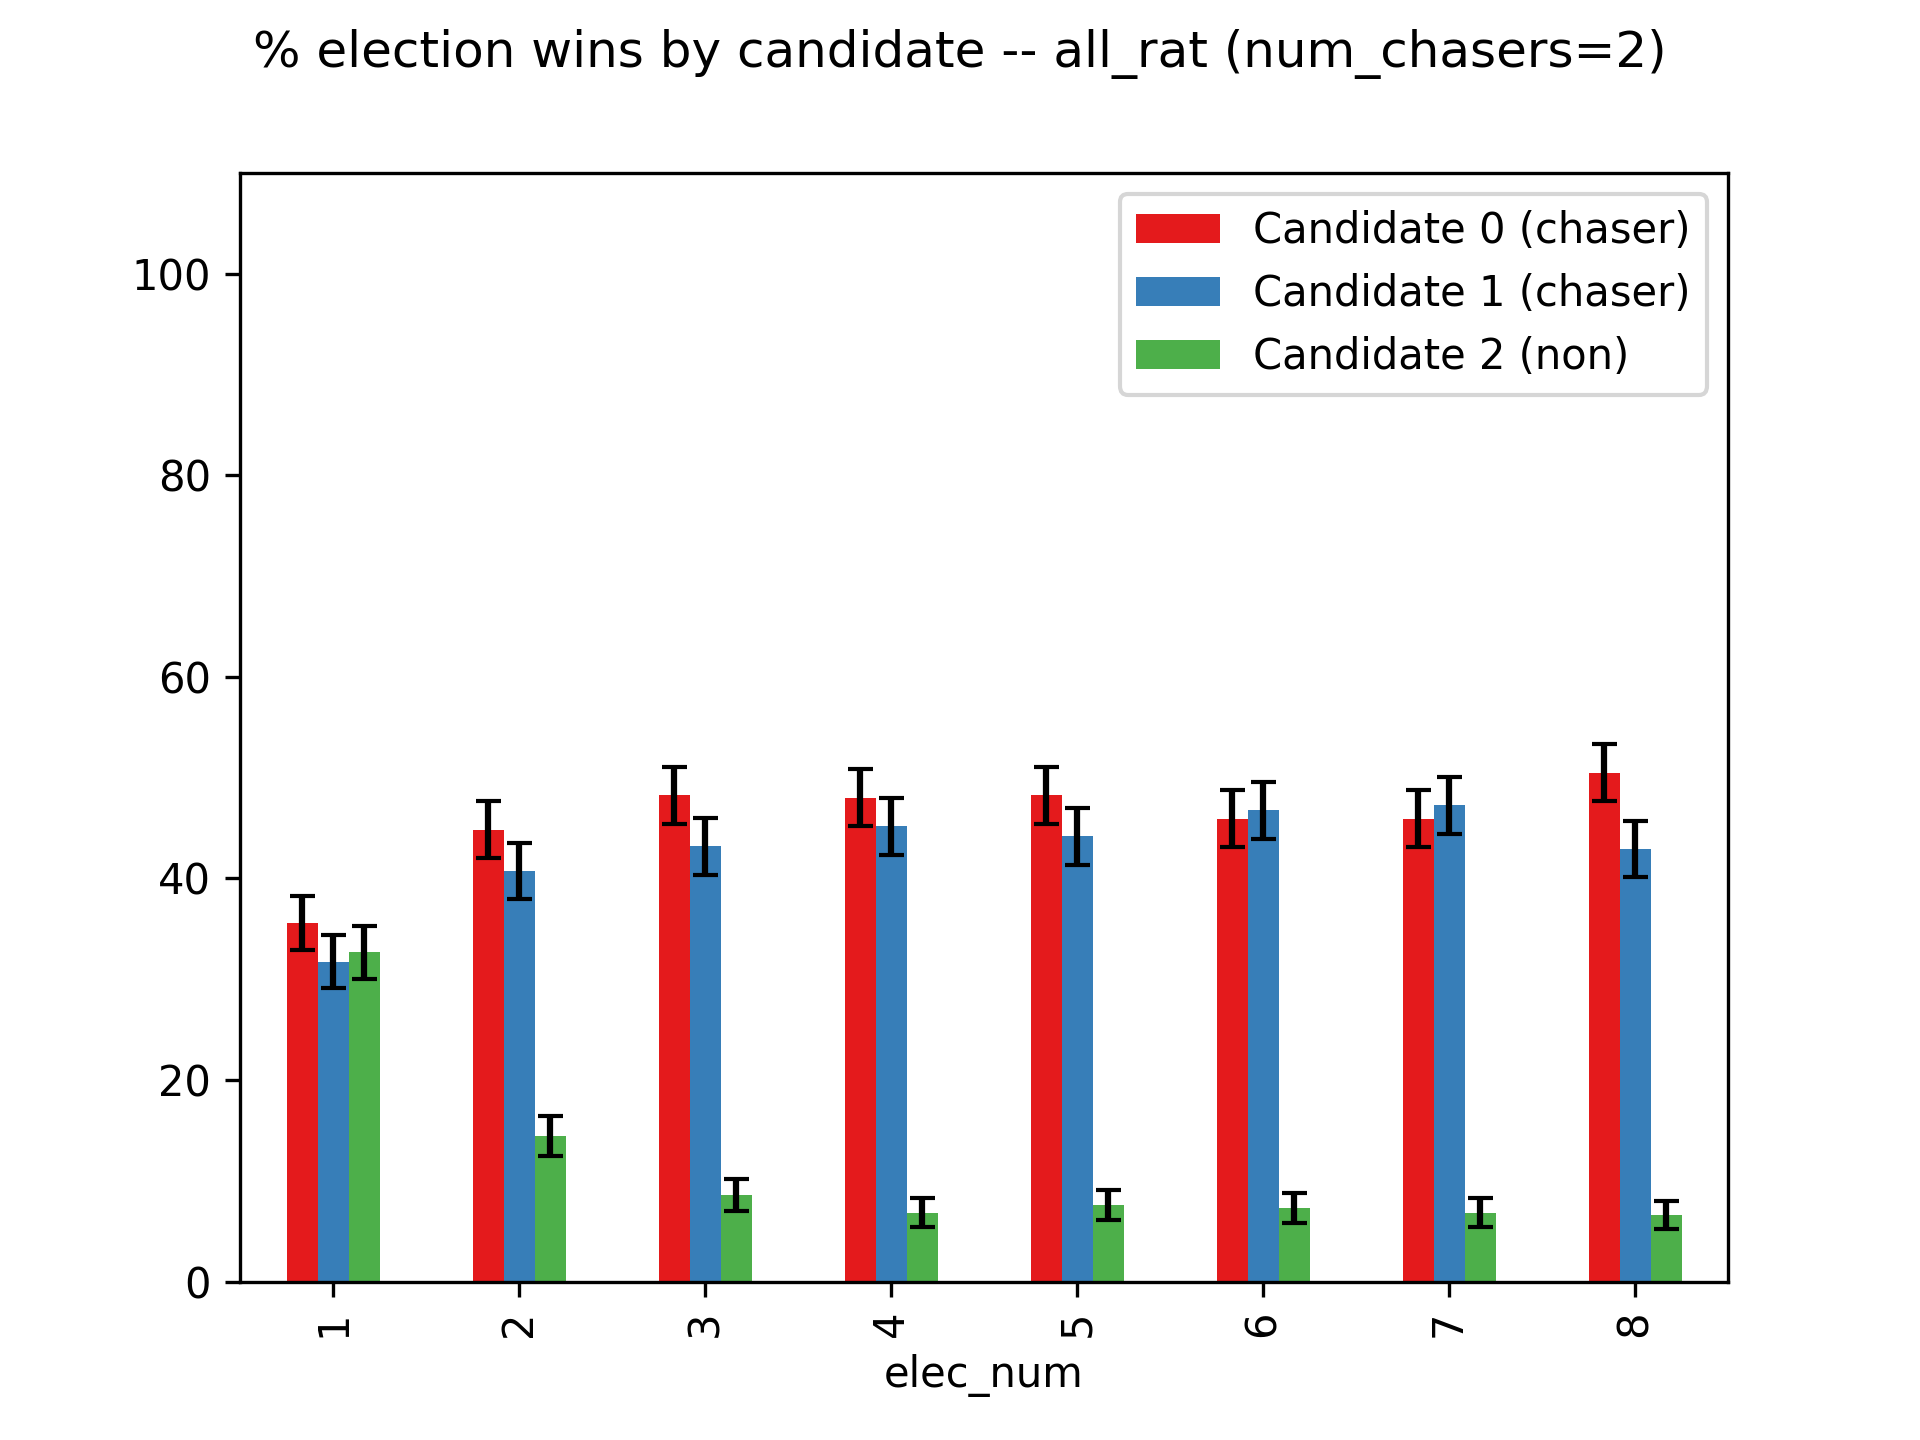
\includegraphics[width=0.45\textwidth]{assets/all_rat_two_chasers_even_bigger_benefit.png}
\caption{An electorate of all rational voters confers maximum benefit to
chasing. Even when there are two chasers (right side) they each receive an
advantage.}
\label{all_rat_chasers_benefit}
\end{figure}

<<<<<<< HEAD
\subsection{The rationality of election outcomes}

Now, using an electorate of all party-line voters, we can measure the impact of
blind party voters on the rationality of election outcomes. An election is considered 
rational if the candidate who actually wins is the same candidate who would have 
won if all agents had voted rationally.
 
Despite the fact that
party affiliations are in line with voter and candidate opinions, voters'
stubbornness in remaining with their parties, as modeled modestly by the party switch
threshold, becomes detrimental to the rationality of elections.
Figure~\ref{all_party_hurt_rat} (left) shows that when no candidates are chasing votes and all 
agents are party-line voters, approximately 60\% of elections are rational. 

More so, when candidates are chasing party-line voters, not only does it fail to provide an 
advantage (as determined above), but it actually decreases the rationality of elections 
(Figure~\ref{all_party_hurt_rat}, right side).

\begin{figure}[ht]
\centering
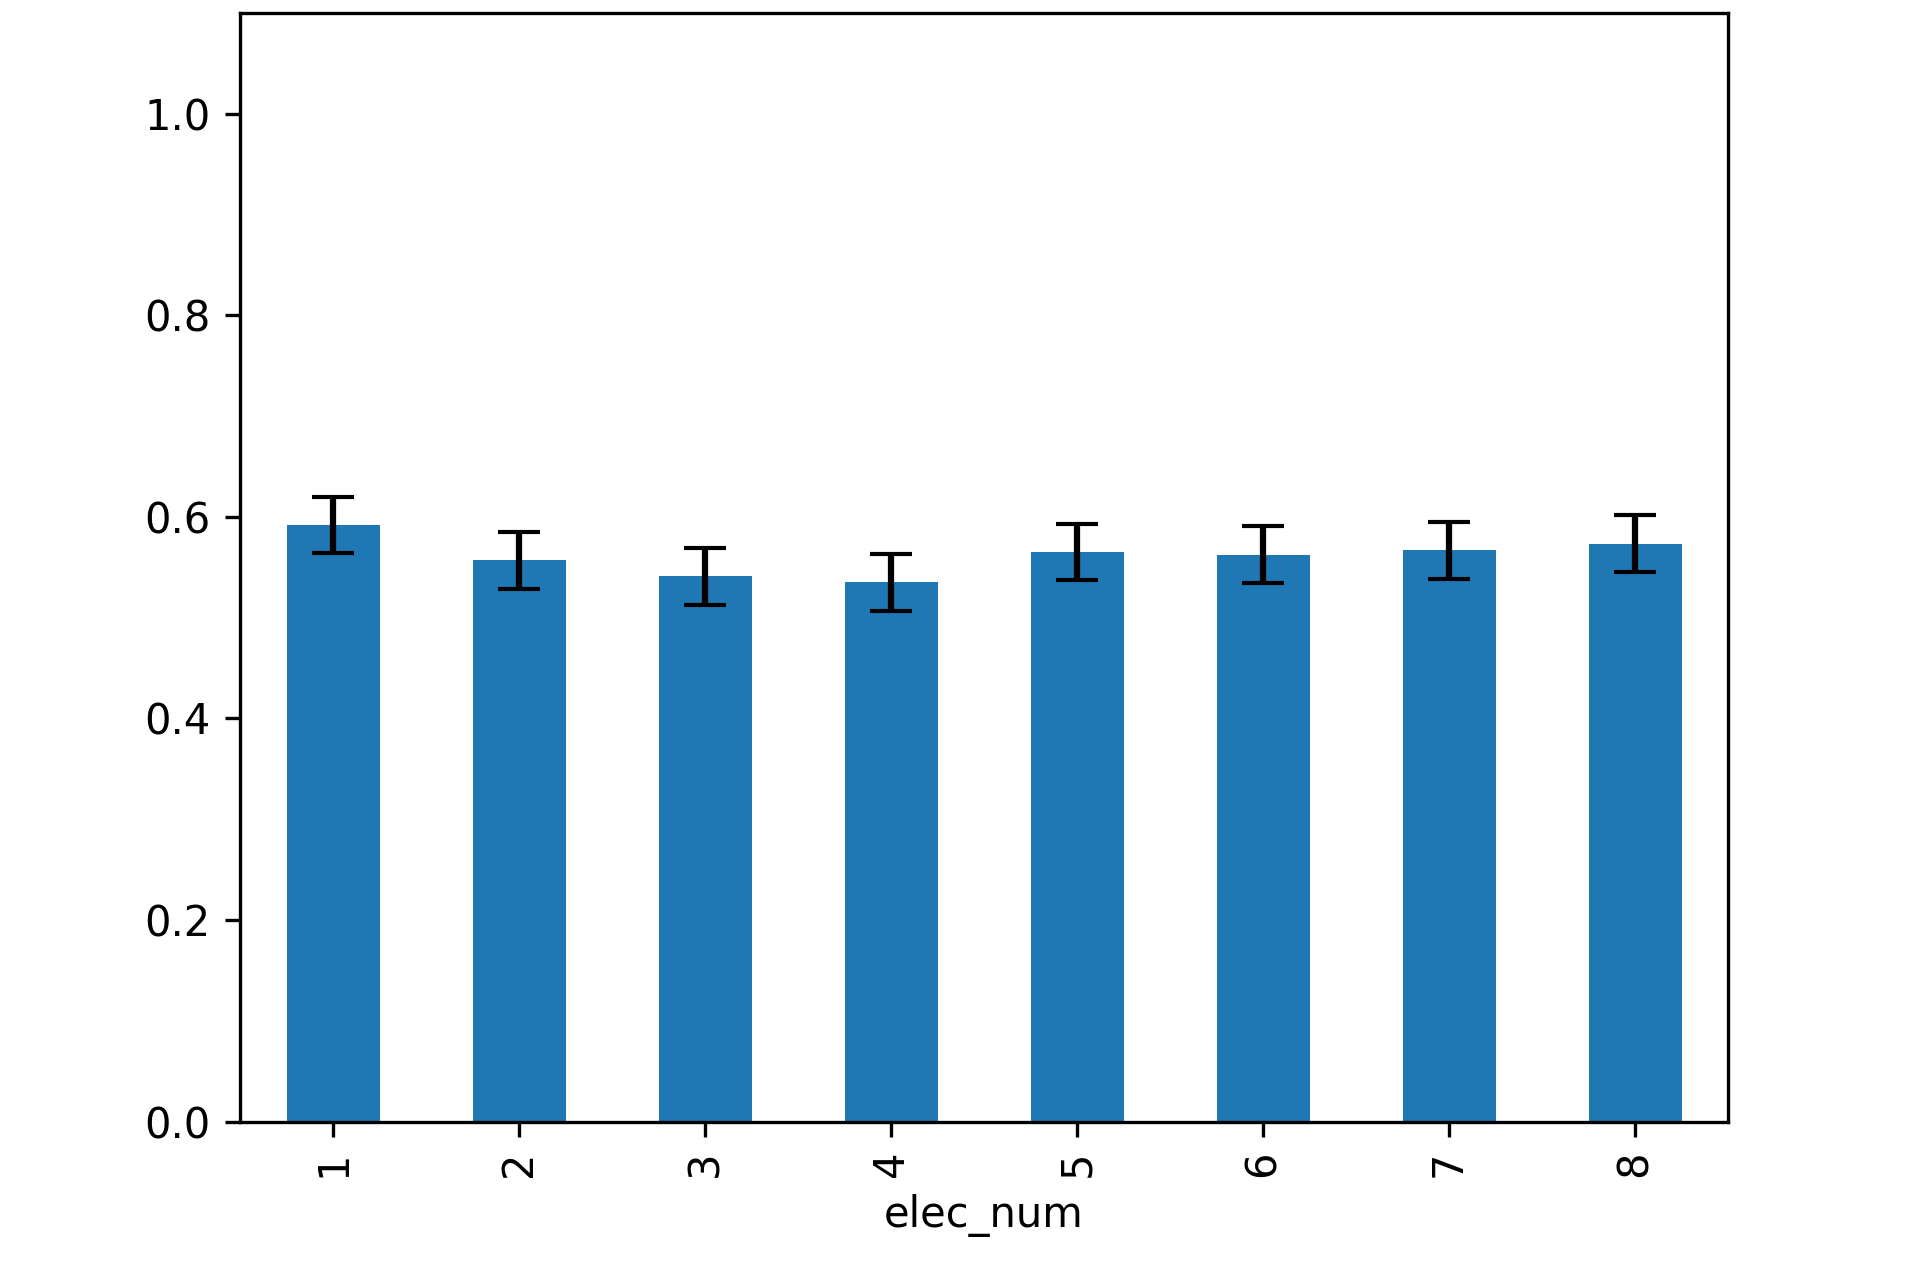
\includegraphics[width=0.45\textwidth]{assets/all_party_0_chasers_rationality_stays_same.png}
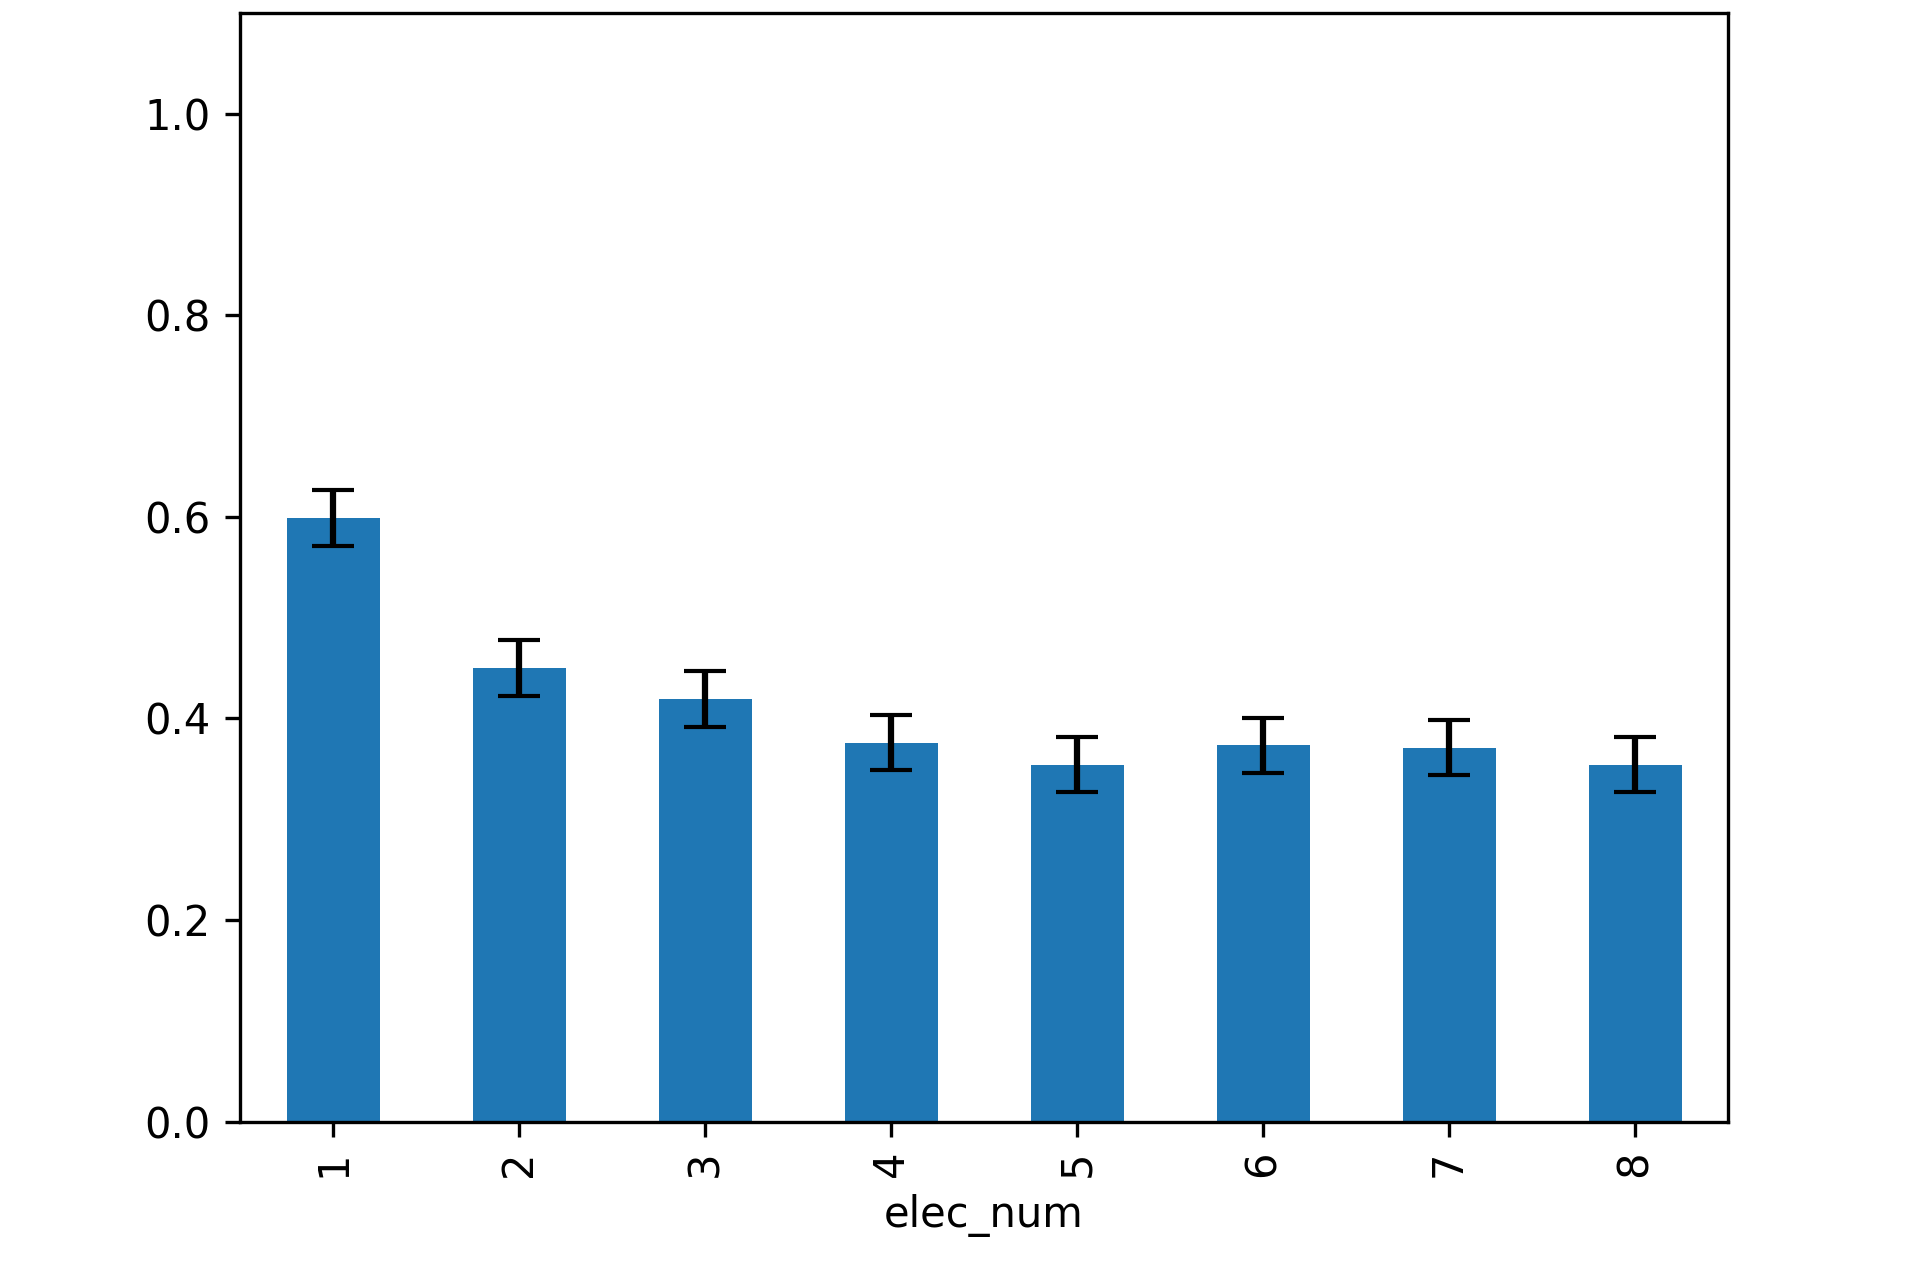
\includegraphics[width=0.45\textwidth]{assets/all_party_3_chasers_rationality_decreases.png}
	\caption{The percentage of rational election outcomes with an electorate of all party-line voters 
	remains constant when there are zero chasing candidates (left), but decreases with three chasing
	candidates (right).}
	\label{all_party_hurt_rat}
=======

\subsection{The chase radius}

Recall that the chase radius sets a limit on how far candidates can wander in
opinion space every time they chase voters. Interestingly, the value of this
parameter has little effect on election outcomes. Figure~\ref{chase_radius}
shows winner outcomes in two-chaser elections for three different values of the
chase radius (the same value is shared by both chasing candidates): 0.1, 0.2,
and 0.3.

\begin{figure}[ht]
\centering
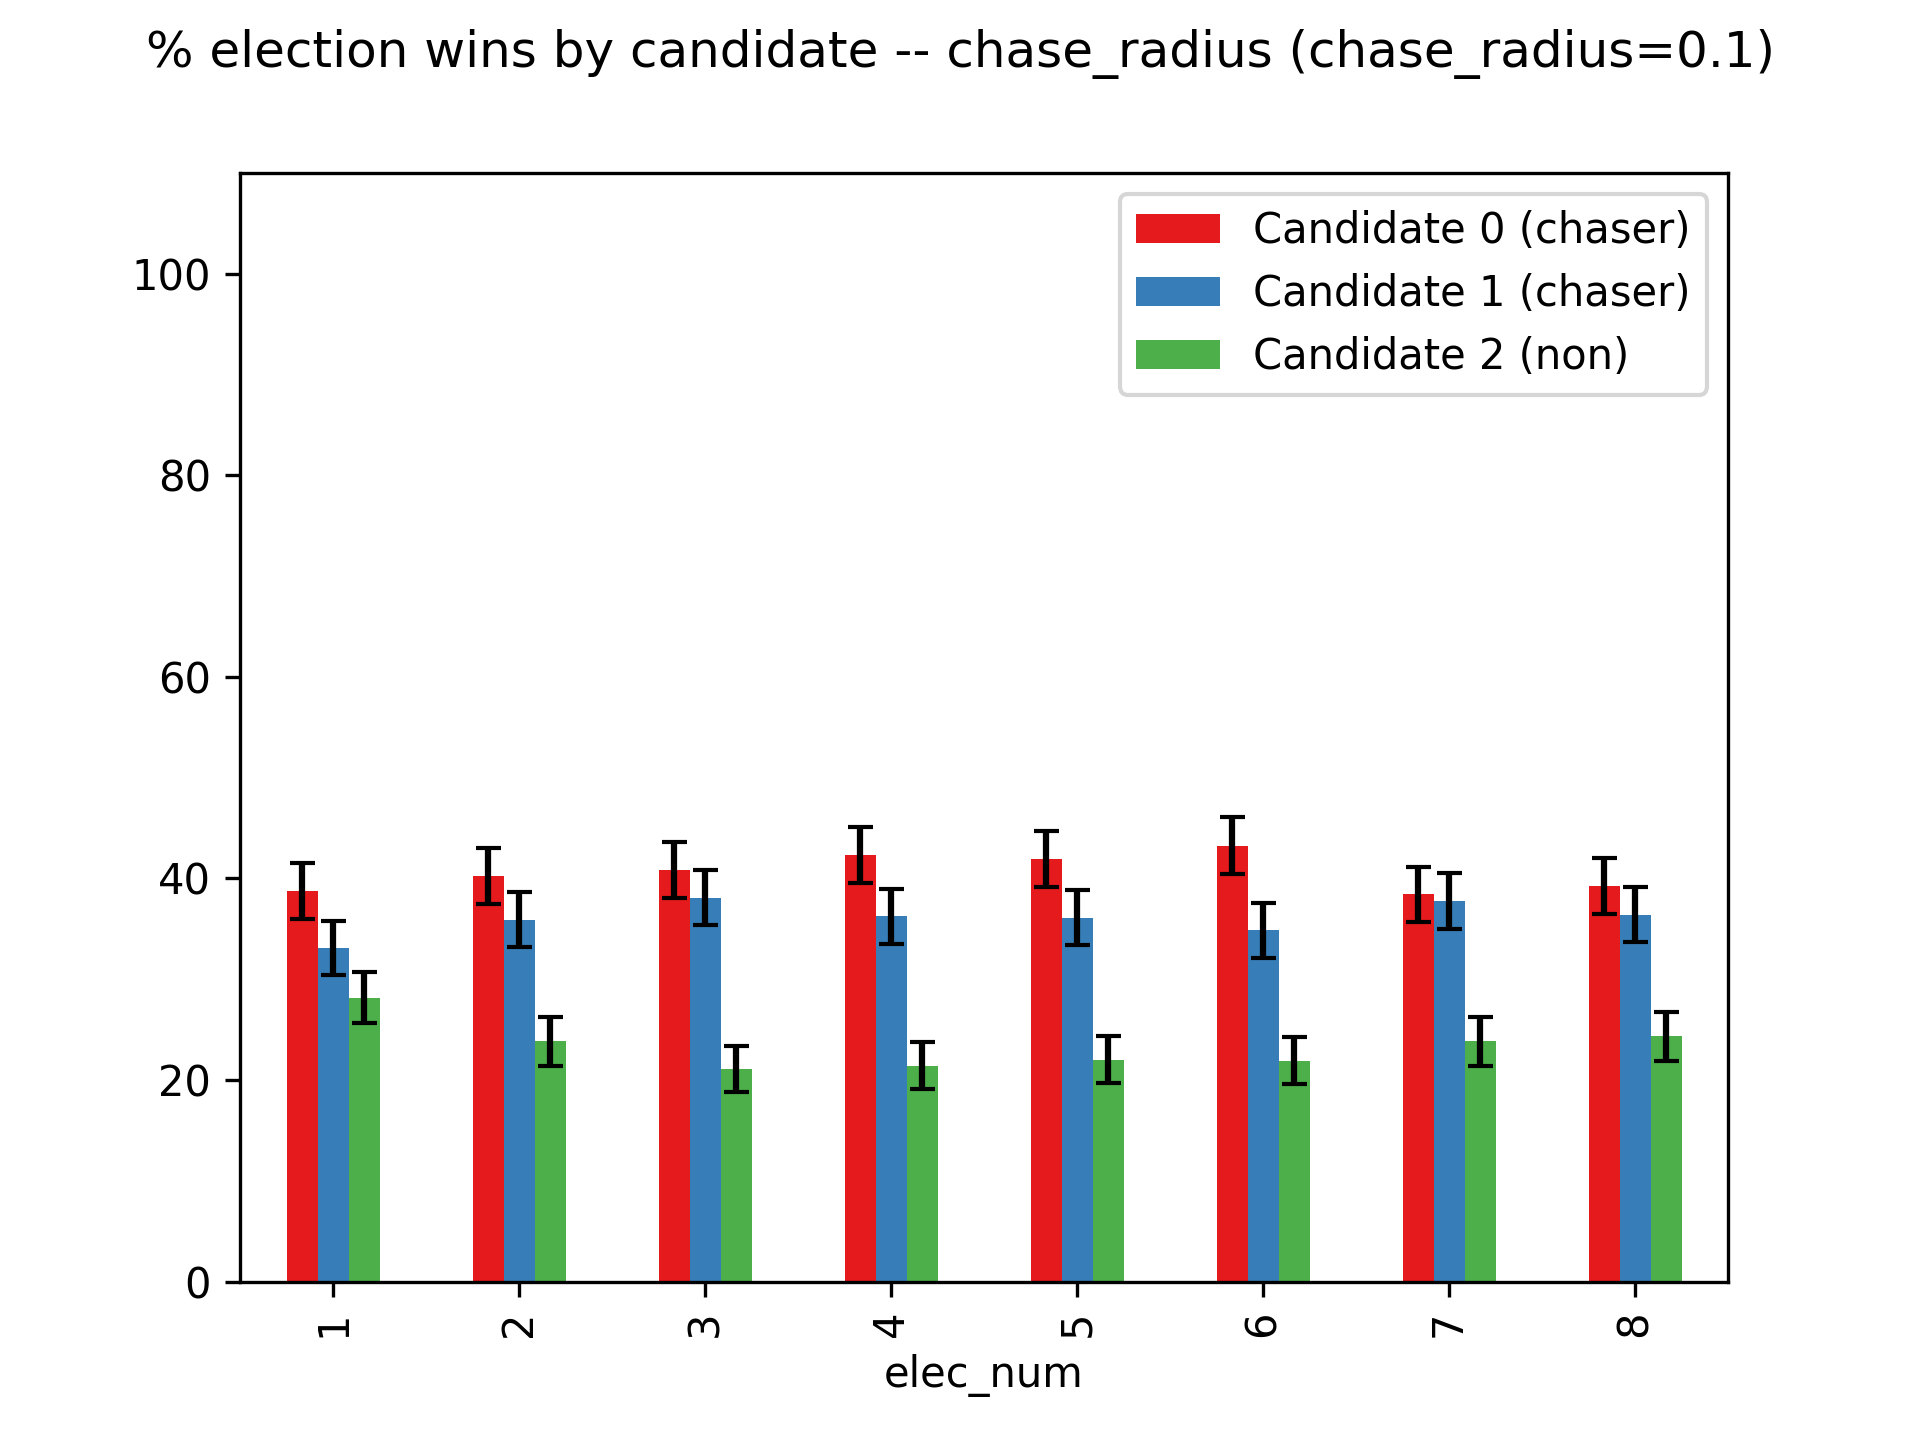
\includegraphics[width=0.31\textwidth]{assets/chase_radius_.1_winners.png}
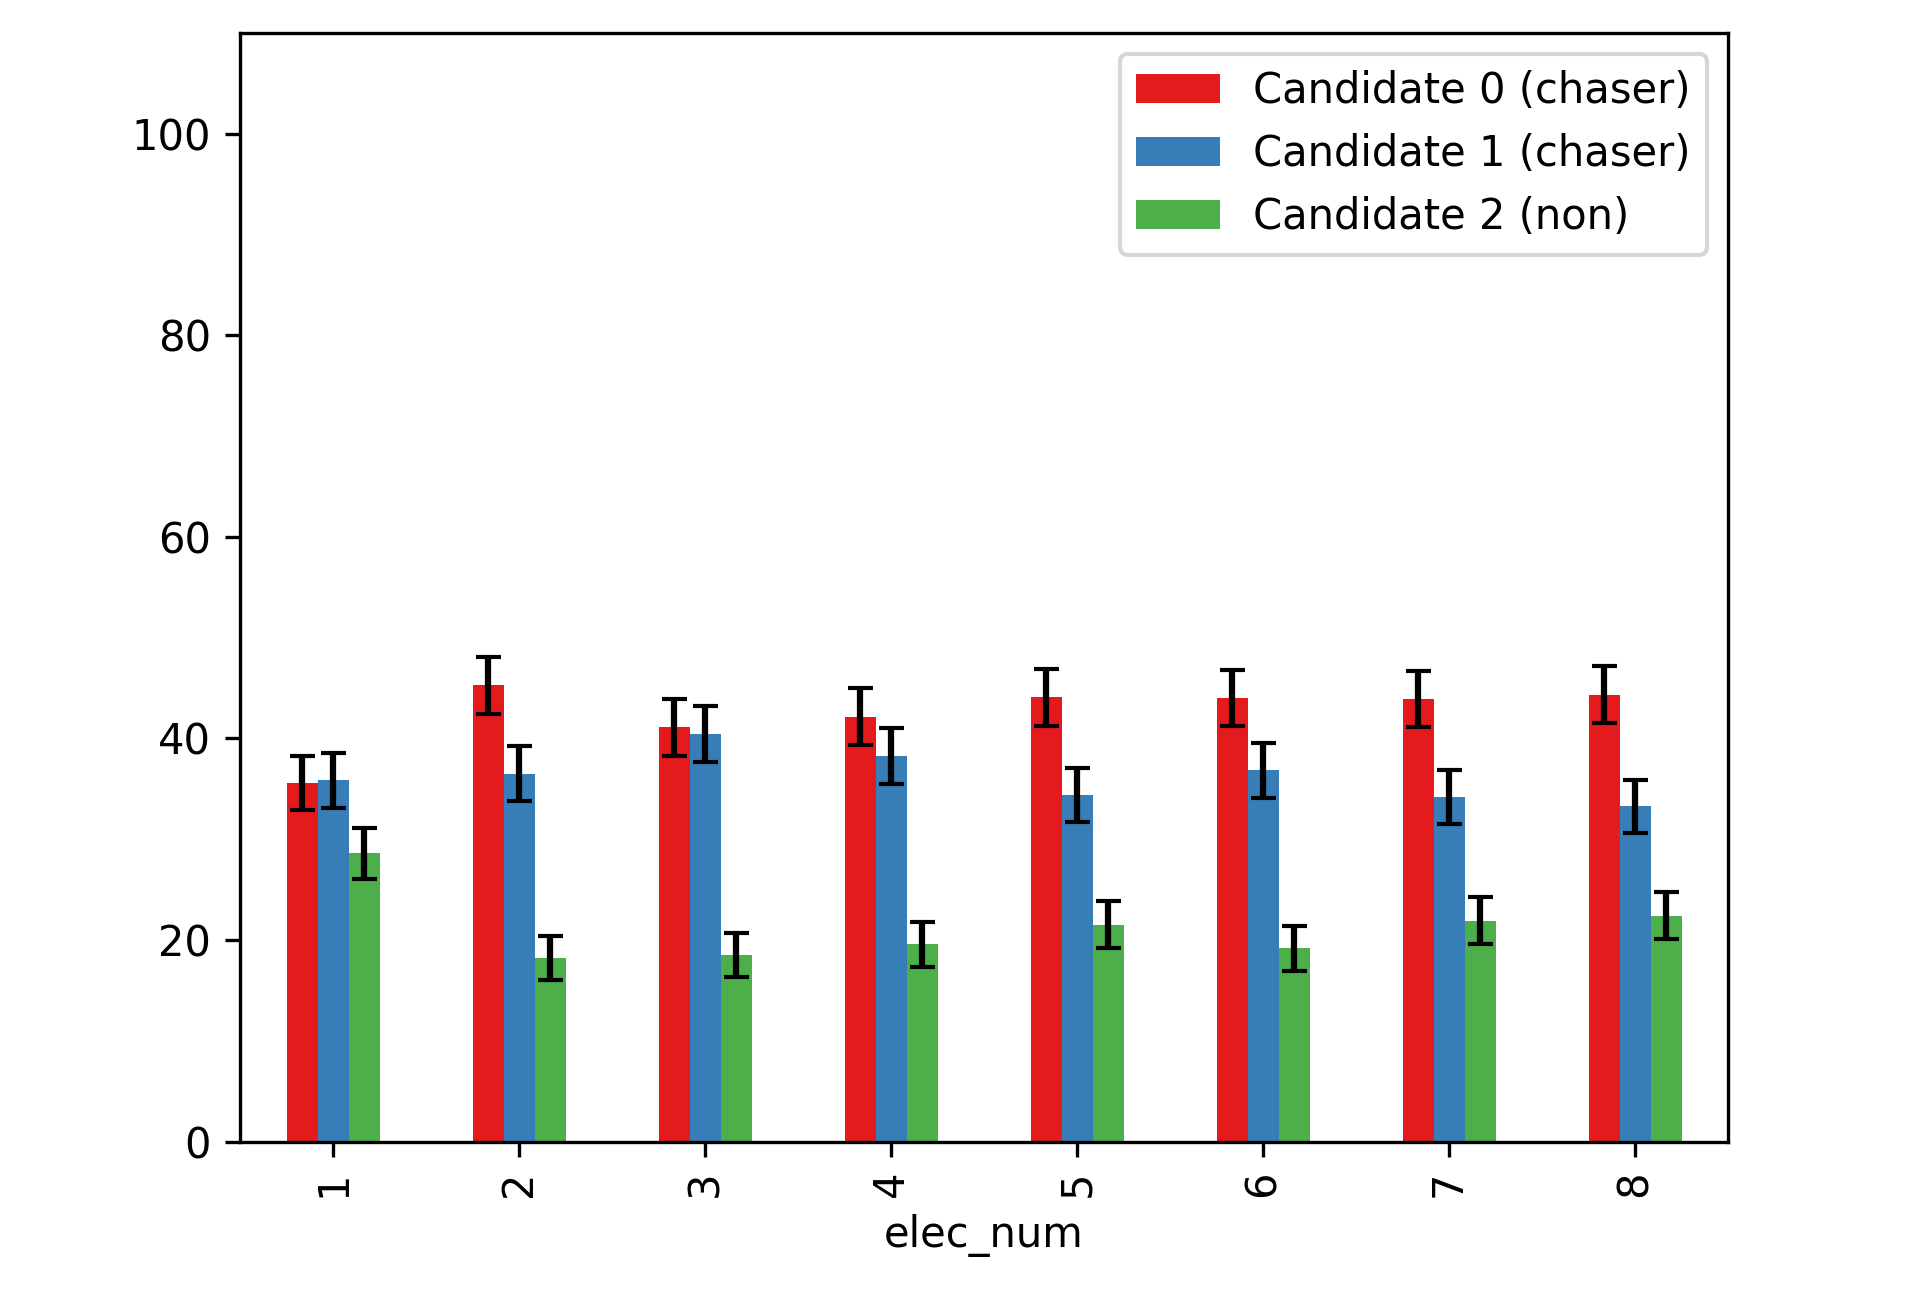
\includegraphics[width=0.31\textwidth]{assets/chase_radius_.2_winners.png}
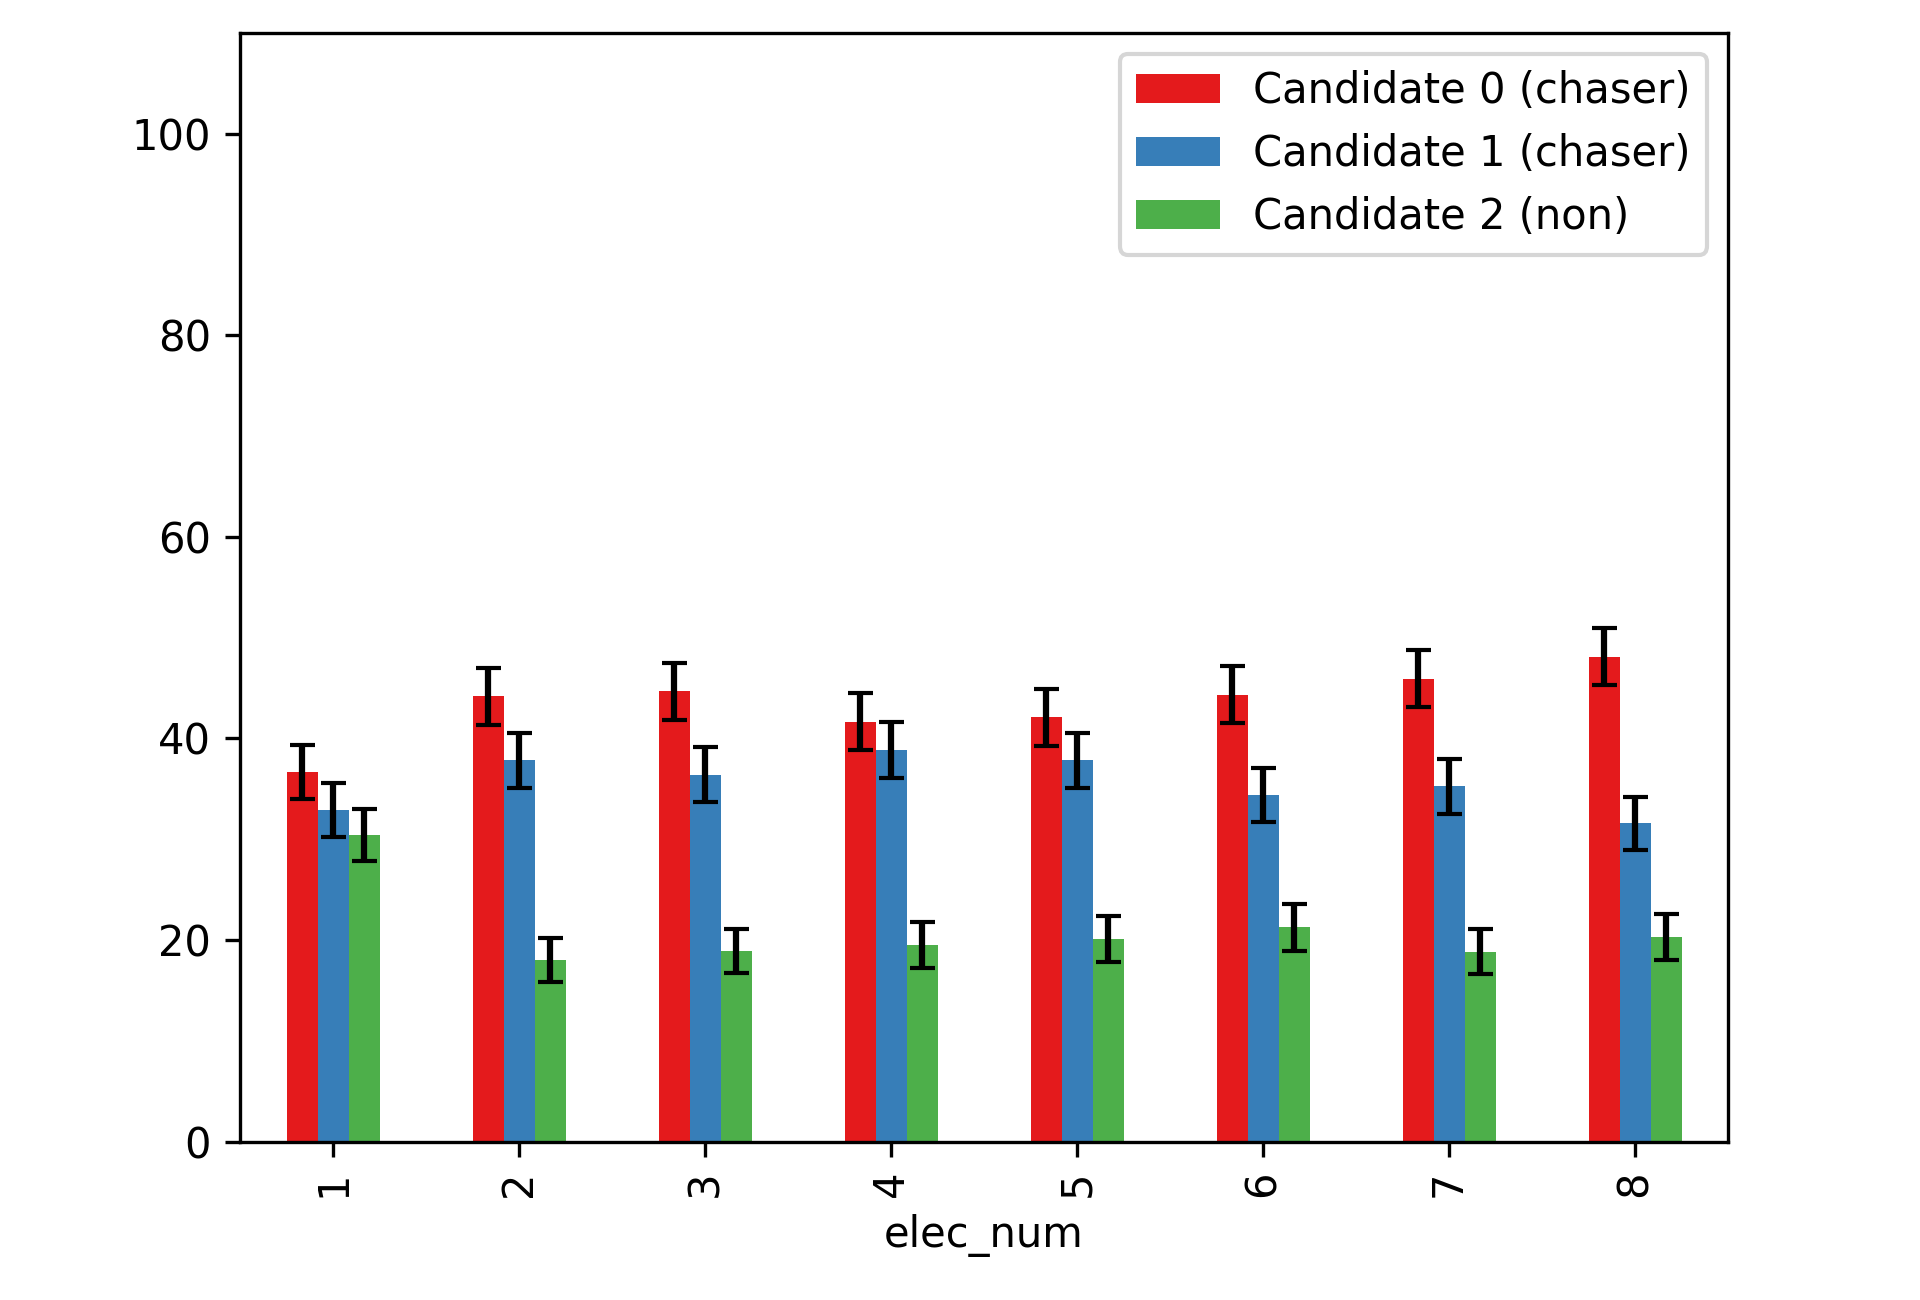
\includegraphics[width=0.31\textwidth]{assets/chase_radius_.3_winners.png}
\caption{Election winners when two chasers' chase radii are varied from .1 to
.2 to .3. The outcomes show negligible difference.}
\label{chase_radius}
\end{figure}

More interesting is when we make one chaser more aggressive than the other
(\textit{i.e.} more willing to take risky positions, and perhaps to abandon
their base and traditional platform). Figure~\ref{diff_chase_radius} shows the
chase distances and election win totals for two chasing candidates with
different chase radii: candidate 0's (red) is .1, and candidate 1's (blue) is
.2. As can be seen, at first candidate 1 makes much larger leaps in opinion
space in an effort to appeal to voters, but after six or seven election cycles
approaches candidate 0's distances. In the right half of the figure, we see
that the more aggressively-chasing candidate now ekes out election victories
its rival in all elections but the first, even with candidate 0 being awarded
ties.

\begin{figure}[ht]
\centering
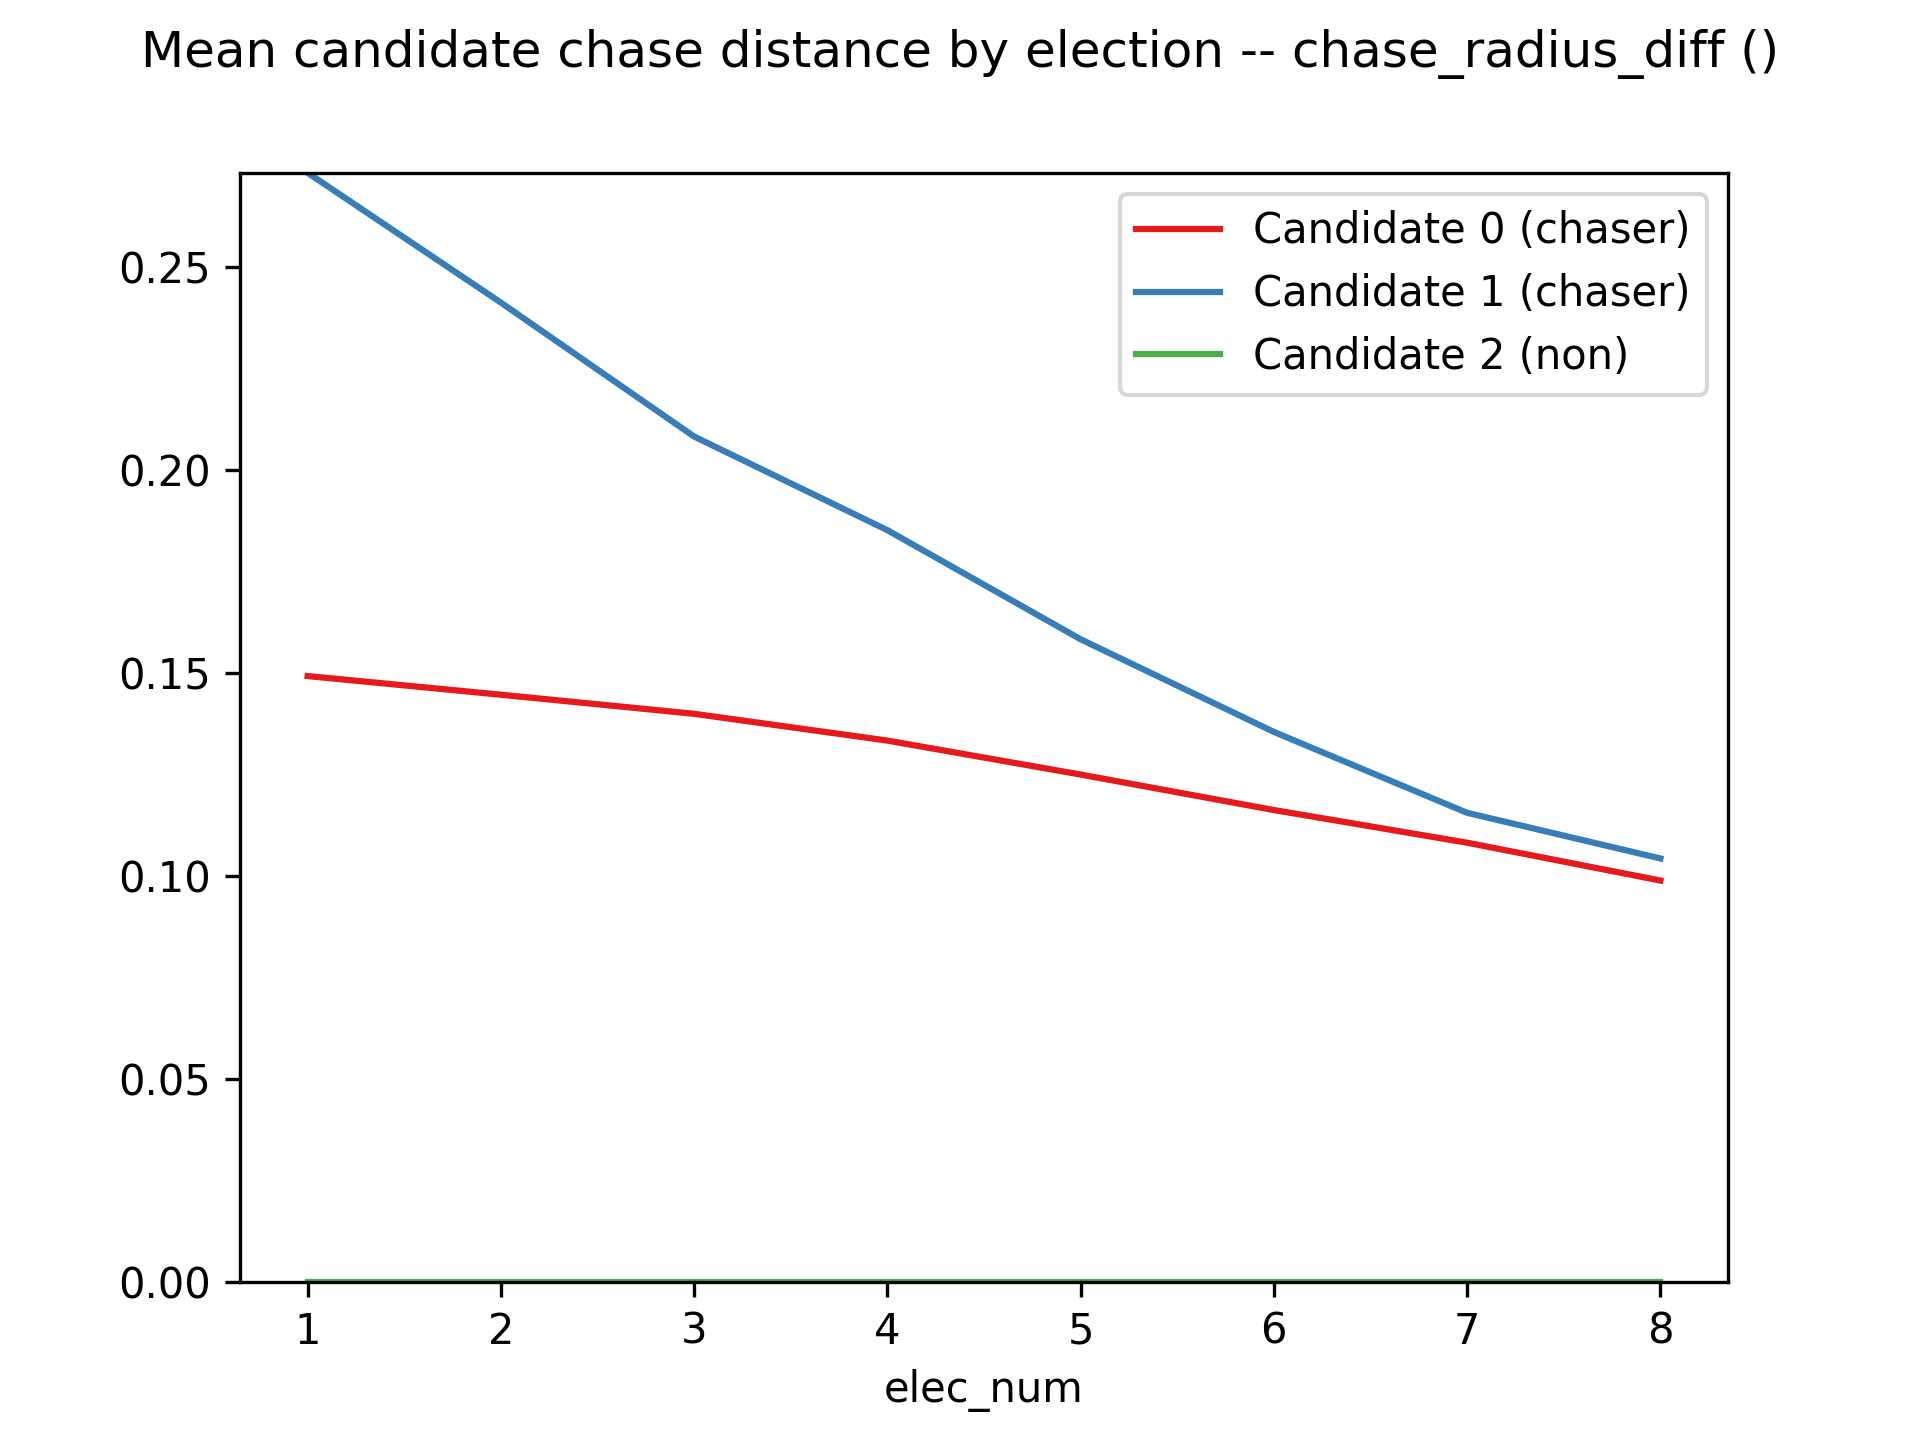
\includegraphics[width=0.45\textwidth]{assets/diff_chase_radii_dists.png}
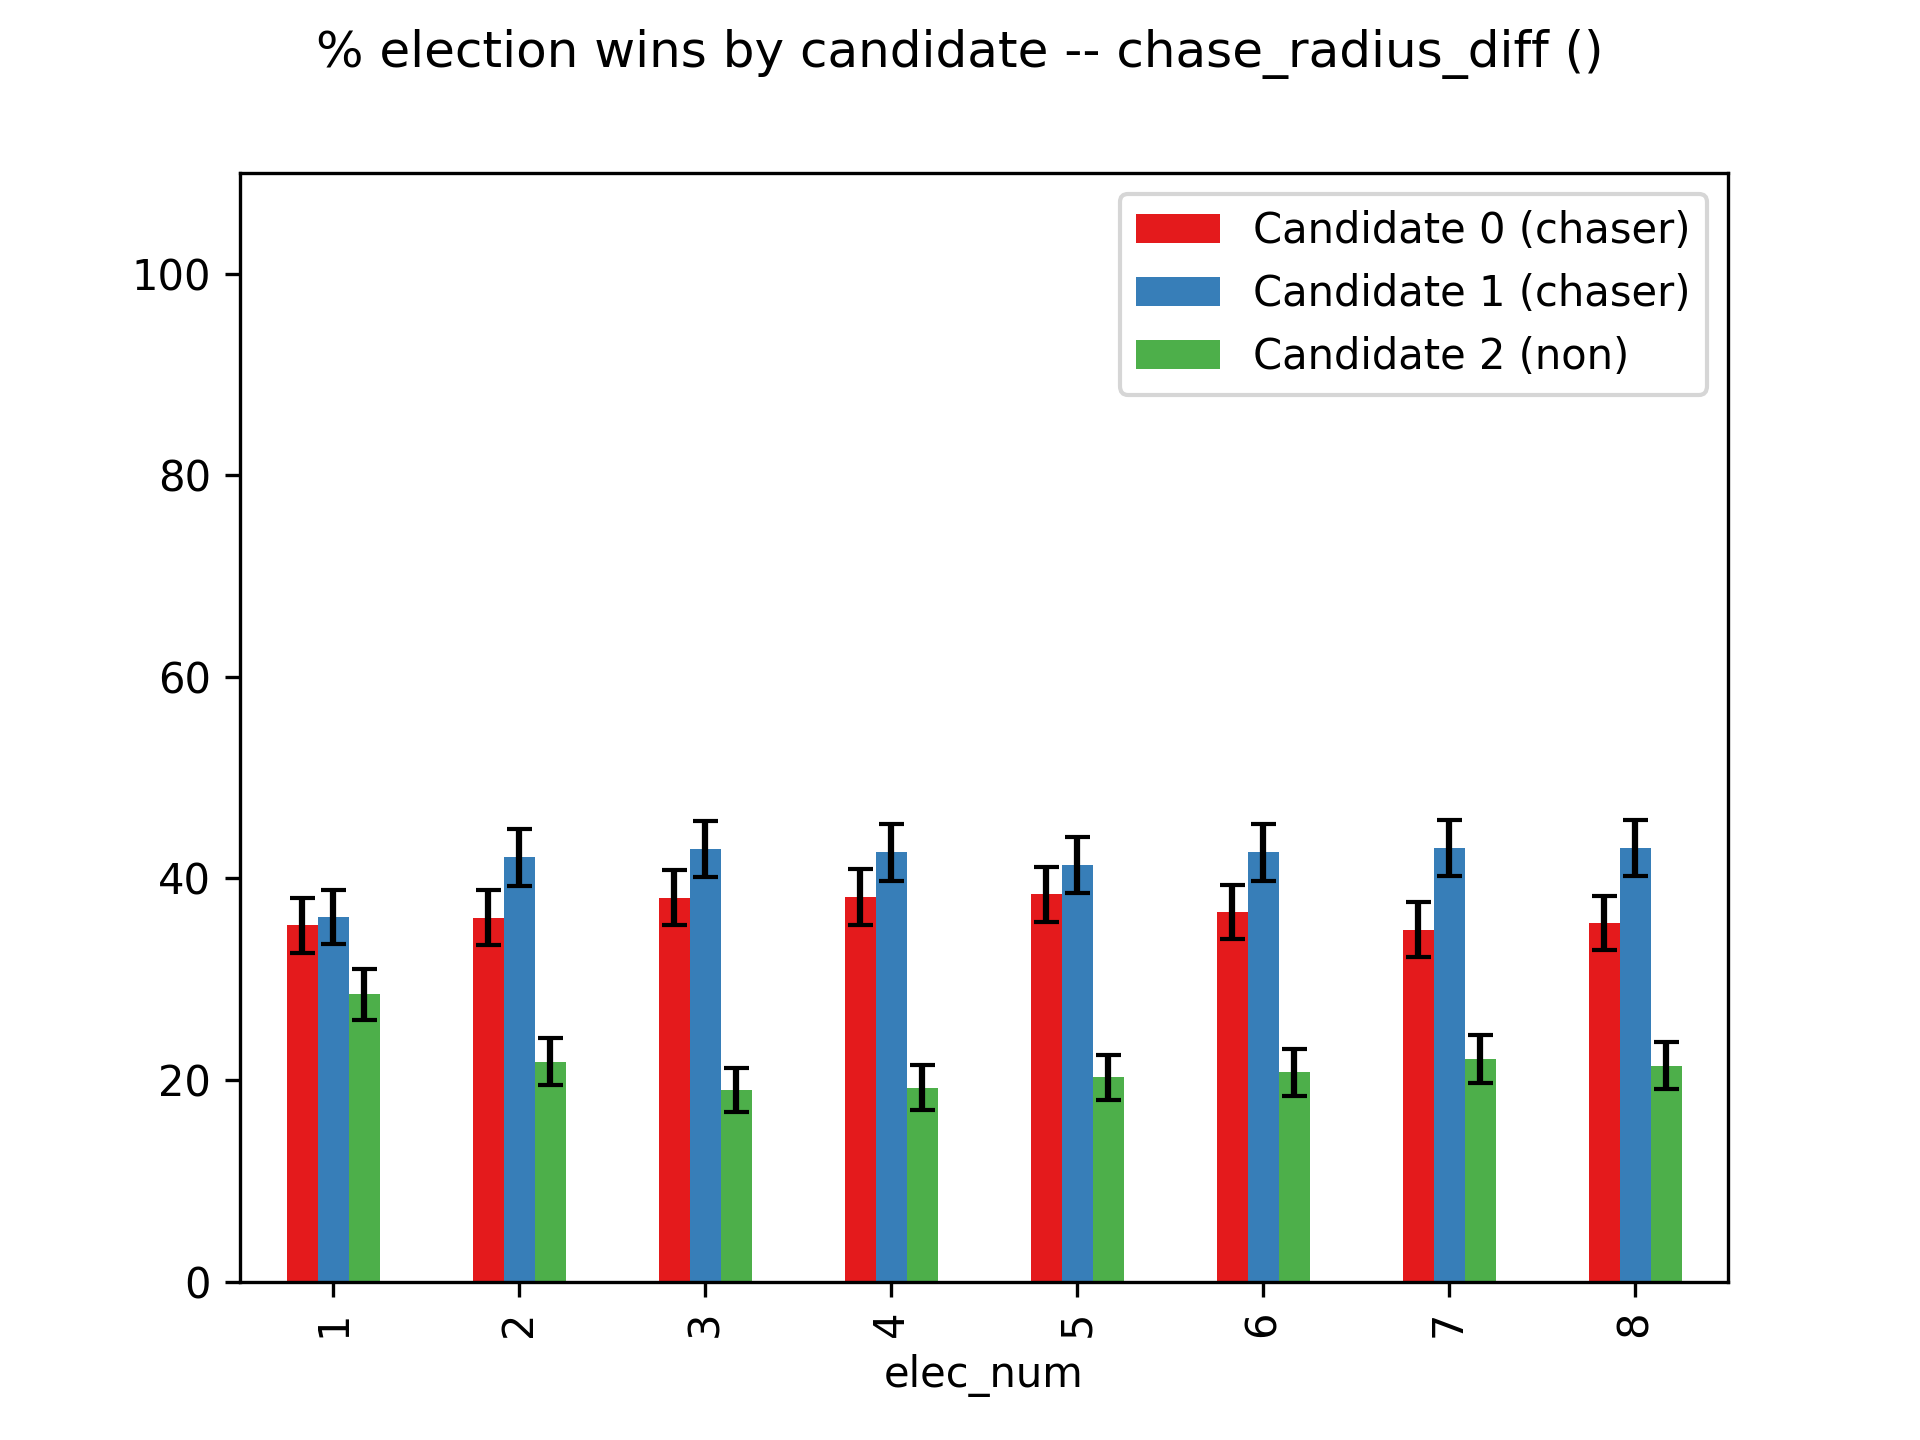
\includegraphics[width=0.45\textwidth]{assets/diff_chase_radii_winners.png}
\caption{Total chase distances, and election outcomes, for two chasing
candidates with different chase radii (candidate 0: radius 0.1; candidate 1:
radius 0.2) plus a non-chasing candidate.}
\label{diff_chase_radius}
>>>>>>> eba78d291079cb29d9ed94f06ce0be7541c452ad
\end{figure}

% Question for us to figure out: why, if default voter alg, only one chaser
% gets any benefit (two chasers cancel each others' benefits out stat sig) but
% if all voters are rational, then two chasers both benefit.


% Some preliminary findings and questions:

% chasing does pay off if lots of rational voters.
% chasing does not pay off if lots of party voters.
% Is there a correlation between how much each candidate chased (total sum of Euclidean distances of all chase actions) and how often they won

% does chasing ever hurt a candidate? hypothesis: if voters easily switch
% parties, and a candidate "overchases" and outruns their base, they will lose
% their base and this will hurt them. Can we reproduce this?

% Is there a correlation between how much the voting population is drifting and how likely the election at that time is to be rational?




